\documentclass[anon]{opt2026} % Author names withheld; switch to \documentclass{opt2026} for the camera-ready version.

% The following packages are automatically loaded by opt2026/jmlr:
% amsmath, amssymb, natbib, graphicx, url, algorithm2e, xcolor, hyperref
% NOTE: amsthm is NOT compatible with jmlr.cls (it raises a ClassError); the
% theorem-like environments below are provided by jmlrutils.sty.

\usepackage[english]{babel}
\usepackage{mathtools}
\usepackage{booktabs}
\usepackage{microtype}
\usepackage{float}

\newtheorem{assumption}[theorem]{Assumption}
\providecommand{\qedhere}{}

\newcommand{\dd}{\mathrm d}
\newcommand{\prefactor}[2]{A_{#1}(#2)}
\DeclareMathOperator*{\argmin}{arg\,min}
\newcommand{\xx}{\mathbf{x}}
\newcommand{\XX}{\mathbf{X}}
\newcommand{\R}{\mathbb{R}}
\newcommand{\E}{\mathbb{E}}

\title[Global Optimization via Softmin Energy Minimization]{Global Optimization via Softmin Energy Minimization}

\optauthor{%
\Name{Samuele Saviozzi} \Email{samuele.saviozzi@phd.unipi.it}\\
\addr Department of Mathematics, University of Pisa, Pisa, Italy
\AND
\Name{Andrea Agazzi} \Email{andrea.agazzi@unibe.ch}\\
\addr Institute of Mathematical Statistics and Actuarial Science, University of Bern, Bern, Switzerland
\AND
\Name{Vittorio Carlei} \Email{carlei@unich.it}\\
\addr Department of Business Economics, University Gabriele d'Annunzio, Chieti, Italy
\AND
\Name{Marco Romito} \Email{marco.romito@unipi.it}\\
\addr Department of Mathematics, University of Pisa, Pisa, Italy
}

\begin{document}

\maketitle

\begin{abstract}
    Non-convex optimization in high dimensions requires balancing gradient information with global exploration, a tension that Langevin dynamics and other gradient-informed methods address only partially. We introduce a gradient-based swarm method driven by a Softmin energy interaction $J_\beta(\xx)$, a smooth approximation of the minimum over the ensemble that couples particles through their relative energies. Combining the resulting gradient flow with Brownian noise, we obtain a dynamics that retains the efficiency of gradient steps while inheriting the global-search behavior of swarm methods. We show that this interaction always partitions the ensemble into particles descending toward local minima and particles automatically repelled toward maxima, and that the same interaction caps the Freidlin--Wentzell quasipotential barrier separating adjacent basins at a level of order $1/\beta$, independently of the true barrier height, strictly below the barrier faced by an overdamped Langevin particle in the same landscape. Numerical experiments on double-well, quadruple-well, and Lennard-Jones cluster benchmarks confirm the analysis and show improved reliability over Simulated Annealing, Langevin dynamics, and variants of Particle Swarm Optimization and Consensus Based Optimization; a high-dimensional Ackley benchmark marks the limit of the approach, where Particle Swarm Optimization is decisively faster.
\end{abstract}

\section{Introduction}
\label{sec:intro}

Non-convex optimization problems are notoriously difficult, since multiple local minima can trap gradient-based algorithms, a central bottleneck across deep learning and reinforcement learning, though the benchmarks in this paper (Section~\ref{sec:numerical-experiments}) target structured, analytically tractable landscapes rather than these settings directly. A classical remedy adds noise to the dynamics, as in Langevin dynamics \citep{CoffeyKalmykovWaldron2004} and noise-perturbed stochastic gradient descent \citep{fehrman2020convergence}, but the mean escape time from a basin grows exponentially in its barrier height \citep{berglund2011kramers}. Multi-particle extensions, including Simulated Annealing \citep{kirkpatrick1983optimization,gelfand1990sampling,tang2024discrete}, Interacting Particle Langevin Dynamics \citep{akyildiz2025interacting,encinar2025proximal}, gradient-based swarm methods \citep{riedl2023gradient,bolte2024swarm,carrillo2021consensus,noel2012new}, and the wider family of Metaheuristics \citep{bandaru2016metaheuristic,yang2020nature}, improve on this by exploring in parallel, but typically either couple particles only through averaging or lack the rigorous guarantees available to gradient methods \citep{hussain2019metaheuristic,rajwar2023exhaustive}.

We introduce a gradient-based swarm method driven by the Softmin energy interaction $J_\beta(\xx)$ (Equation~\eqref{eq:Softmin-energy}), a smooth approximation of the empirical minimum over an ensemble of particle values that couples particles through their relative energies (Section~\ref{sec:method}). We prove two guarantees.

\paragraph{Dynamic ensemble partitioning and accelerated convergence.} The interaction $\nabla J_\beta$ partitions the ensemble via a state-dependent effective learning rate $\prefactor{k}{\xx}$ (Equation~\eqref{eq:pre-factor}): at every stable equilibrium, at least one particle sits at a local minimum while trapped, high-energy particles are automatically repelled to hill-climb and explore (Theorem~\ref{thm:stationary-points}). The ensemble's running best objective value is always nonincreasing, and, under a Polyak--\L{}ojasiewicz condition, converges to the global minimum at least as fast as ordinary gradient flow, for any inverse-temperature schedule (Theorem~\ref{thm:ensemble-min}).

\paragraph{Provable barrier flattening.} At fixed temperature, the same interaction caps the Freidlin--Wentzell quasipotential barrier separating adjacent basins at a level of order $1/\beta$, independently of the true barrier height, strictly below the exact small-noise exit exponent of an overdamped Langevin particle in the same landscape (Theorem~\ref{thm:barrier-cap-main}; full three-part statement and proof as Theorem~\ref{thm:transition-time} in Appendix~\ref{apx:barrier-full}).

Our method differs from Consensus-Based Optimization, Particle Swarm Optimization, and other metaheuristics \citep{CarrilloChoiTotzeckTse2018,fornasier2024consensus,pinnau2017consensus,carrillo2021consensus,kennedy1995particle,noel2012new,Goldberg1989,DorigoStutzle2004} in using the Softmin energy of particle values as the \emph{sole} source of interaction: unlike consensus-based averaging or the log-sum-exp free energy $F_\beta(\xx)=-\beta^{-1}\log\sum_ie^{-\beta f(x_i)}$, whose gradient strictly preserves the sign of ordinary gradient descent, this explicitly assigns each particle a minimizing or maximizing role. It is closer in spirit to Interacting Particle Langevin Dynamics \citep{akyildiz2025interacting,encinar2025proximal} in relying on genuine ensemble-level coupling rather than independent copies, but couples particles through their relative energies rather than an empirical average, and targets global optimization of $f$ rather than marginal-likelihood estimation. To our knowledge this is the first use of $J_\beta$ itself as an optimization objective, and the barrier-flattening mechanism of Theorem~\ref{thm:barrier-cap-main} is previously unstudied. Appendix~\ref{apx:related-work} gives the full comparison, including to Population Annealing \citep{Wang_2015} and to theoretical work on the Softmin/Boltzmann operator \citep{bertsekas1999nonlinear,mei2020global,song2019revisiting}.

Section~\ref{sec:numerical-experiments} tests these predictions on double-well, quadruple-well, and Lennard-Jones cluster benchmarks against seven baselines, and reports a high-dimensional Ackley benchmark as the honest boundary of the approach, where Particle Swarm Optimization is decisively faster. Proofs are deferred to Appendix~\ref{apx:technical-proofs}; experimental details to Appendix~\ref{app:hyperparameters}.

\section{Method and Theoretical Guarantees}
\label{sec:method}

Consider a differentiable function $f:\R^d\to\R$ and a population of $n$ particles $\xx=(x_1,\dots,x_n)$, $x_i\in\R^d$. The Softmin energy of the ensemble is
\begin{equation}
    J_\beta(\xx)=\sum_{i=1}^n\frac{\exp(-\beta f(x_i))}{\sum_{j=1}^n\exp(-\beta f(x_j))}f(x_i),
    \label{eq:Softmin-energy}
\end{equation}
a smooth approximation of $\min_if(x_i)$, sharpening as $\beta\to\infty$ and recovering the ensemble average as $\beta\to0$. We consider the stochastic gradient flow
\begin{equation}\label{e:sde}
   \dd\xx_t = -n\nabla J_{\beta_t}(\xx_t)\dd t+\sqrt{2\sigma}\dd B_t,
\end{equation}
where $(B_t)$ is a standard $nd$-dimensional Brownian motion, $\sigma>0$ drives exploration, and $\beta_t>0$ may vary over time (Theorem~\ref{thm:ensemble-min} holds for an arbitrary schedule; the barrier analysis of Section~\ref{sec:method-barrier} fixes $\beta$). Writing $w_k=e^{-\beta f(x_k)}(\sum_je^{-\beta f(x_j)})^{-1}$ for the Gibbs weight of $x_k$, the dynamic pre-factor is
\begin{equation}
    \prefactor{k}{\xx}=nw_k\bigl[1-\beta(f(x_k)-J_\beta(\xx))\bigr],
    \label{eq:pre-factor}
\end{equation}
and the gradient of $nJ_\beta$ satisfies
\begin{equation}
    \nabla_{x_k} (nJ_\beta(\xx)) =\prefactor{k}{\xx} \nabla f(x_k), \qquad \sum_{k=1}^n \prefactor{k}{\xx} = n,
    \label{eq:softmin-gradient}
\end{equation}
so \eqref{e:sde} reads componentwise as $\dot x_k=-\prefactor{k}{\xx}\nabla f(x_k)+\text{noise}$: each particle performs a gradient step on $f$ scaled by its own state-dependent, sign-changing \emph{effective learning rate} $\prefactor{k}{\xx}$. When $f(x_k)<J_\beta(\xx)+1/\beta$ the pre-factor is positive and the particle minimizes; otherwise it is negative and the particle is driven uphill. Since $\sum_k\prefactor{k}{\xx}=n$, at least one pre-factor is always strictly positive.

\begin{theorem}[Stationary points]
    \label{thm:stationary-points}
    Let $f\in C^2(\R^d)$, $\beta>0$, and let $\bar\xx=(\bar x_1,\dots,\bar x_n)$ be a locally asymptotically stable equilibrium of $\dd\xx_t=-n\nabla J_\beta(\xx_t)\dd t$. Then for every $k$, evaluated at $\bar\xx$: $\nabla f(\bar x_k)=0$; $\prefactor{k}{\bar\xx}\ne0$; and $\prefactor{k}{\bar\xx}>0$ (equivalently $f(\bar x_k)<J_\beta(\bar\xx)+1/\beta$) iff $\bar x_k$ is a local minimum of $f$, while $\prefactor{k}{\bar\xx}<0$ iff $\bar x_k$ is a local maximum. In particular, at least one particle sits at a local minimum of $f$.
\end{theorem}

A sufficient Hessian-sign condition guaranteeing such an equilibrium is stable, and a global-existence argument for the noisy dynamics, are given in Appendix~\ref{apx:technical-proofs}. Theorem~\ref{thm:stationary-points} shows the deterministic flow can stabilize at particles sitting simultaneously at minima and maxima of $f$; which equilibrium is reached depends on initialization, motivating the noise in \eqref{e:sde} as an escape mechanism (Section~\ref{sec:method-barrier}).

\begin{definition}[Polyak--\L{}ojasiewicz condition]
    \label{def:pl-condition}
    $f:\R^d\to\R$ satisfies the \emph{PL condition} on $S\subseteq\R^d$ with constant $\mu>0$ if $\tfrac12\|\nabla f(x)\|^2\ge\mu(f(x)-f_\star)$ for every $x\in S$, where $f_\star:=\inf f$.
\end{definition}

\begin{theorem}[Descent of the ensemble minimum]
    \label{thm:ensemble-min}
    Let $f\in C^1(\R^d)$ have locally Lipschitz gradient, let $\beta_t>0$ be measurable, and let $\xx(t)$ solve $\dot x_k(t)=-\prefactor{k}{\xx(t)}\nabla f(x_k(t))$. Let $m(t):=\min_kf(x_k(t))$. Then $m$ is nonincreasing; if in addition $f$ satisfies the PL condition (Definition~\ref{def:pl-condition}) with constant $\mu>0$ on $S_0:=\{x:f(x)\le m(0)\}$, then
    \[
        m(t)-f_\star\le e^{-2\mu t}\bigl(m(0)-f_\star\bigr), \qquad t\ge0.
    \]
\end{theorem}

Theorem~\ref{thm:ensemble-min} is a no-slowdown guarantee for the ensemble's leading particle: the Softmin coupling never makes the running best value worse than ordinary gradient flow, for \emph{any} inverse-temperature schedule. Proofs of both theorems are in Appendix~\ref{apx:technical-proofs}.

\subsection{Barrier flattening}
\label{sec:method-barrier}

Fixing $\beta_t\equiv\beta$ in \eqref{e:sde} and specializing to $d=1$, consider three consecutive nondegenerate critical points $z_-<s<z_+$ of $f$, with $z_\pm$ local minima, $s$ the separating maximum, and barrier $h:=f(s)-f(z_-)>0$. Freezing $n-1$ particles at $z_-$ and letting one particle move, $\Gamma(x):=(x,z_-,\dots,z_-)$, reduces the dynamics on this invariant channel to a one-dimensional gradient flow on the \emph{reduced potential} $u(r):=nre^{-\beta r}/(n-1+e^{-\beta r})$ of the relative energy $r=f(x)-f(z_-)$ (Appendix~\ref{apx:barrier-full}). This channel gives an explicit, computable upper bound on the Freidlin--Wentzell quasipotential $V_\beta$ governing small-noise exit times \citep{freidlin2012random} (background in Appendix~\ref{apx:fw-theory}).

\begin{theorem}[Barrier flattening, headline bound]
    \label{thm:barrier-cap-main}
    Under the nondegeneracy and monotonicity conditions on $f$ made precise in Assumption~\ref{assum:channel} (Appendix~\ref{apx:barrier-full}), for every $n\ge2$, $\beta>0$,
    \begin{equation}
        u_c:=\max_{r\in\R}u(r)<\frac{n}{e(n-1)\beta}, \qquad\qquad V_\beta\bigl(\Gamma(z_-),\Gamma(s)\bigr)\le u_h<\min\{h,r_c\}\le h,
        \label{eq:barrier-cap}
    \end{equation}
    where $r_c$ is the relative energy at which the active particle switches from minimizing to maximizing and $u_h:=\max_{0\le r\le h}u(r)$. Both $u_c$ and $r_c$ are of order $\beta^{-1}$, uniformly in $h$: the quasipotential separating $z_-$ from the saddle $s$ is capped at a level of order $1/\beta$ for \emph{any} physical barrier height $h$, strictly below the exact exponent $h$ that governs a single overdamped Langevin particle in the same landscape.
\end{theorem}

Theorem~\ref{thm:barrier-cap-main} is the headline case of a full three-part result (post-saddle passage into $z_+$ included) stated and proved as Theorem~\ref{thm:transition-time} in Appendix~\ref{apx:barrier-full}, together with the exact exit-time consequence under metastable-domain hypotheses (Corollary~\ref{cor:exit-time-conditional}), the low-barrier regime, and the extension to $d>1$ and to annealed temperature schedules (Remarks~\ref{rem:low-barrier}--\ref{rem:higher-dim}). This is a $\sigma\downarrow0$ statement; Section~\ref{sec:numerical-experiments} discusses its relation to the $\sigma=1$ regime used in the benchmarks below.

\section{Numerical Experiments}
\label{sec:numerical-experiments}

We compare fixed-$\beta$ ($\beta=10$) Softmin dynamics (Euler--Maruyama discretization of \eqref{e:sde}; full algorithm and hyperparameters in Appendix~\ref{app:hyperparameters}) against seven baselines: Simulated Annealing \citep{gelfand1990sampling}; overdamped Langevin dynamics \citep{welling2011bayesian}; Gradient-Aware Consensus-Based Optimization \citep{carrillo2021consensus}, with and without upward $\beta$-annealing; Gradient-Enhanced Particle Swarm Optimization \citep{noel2012new}; and the canonical, gradient-free forms of both \citep{CarrilloChoiTotzeckTse2018,pinnau2017consensus,kennedy1995particle}. Entry time is measured against a value-space target (0.15 of the benchmark's own depth gap for the wells, $10^{-2}$ above the literature global minimum for Lennard-Jones); each plotted mean is over seeds that reached the target, and a sweep point below a 50\% reached-fraction is omitted rather than plotted from a small surviving sample. One caveat frames everything below: Theorem~\ref{thm:barrier-cap-main} is a $\sigma\downarrow0$ statement, whereas the benchmarks run at $\sigma=1$, where the cap of \eqref{eq:barrier-cap} evaluates to $u_c\approx0.037$, negligible against the noise, so these experiments test whether the Softmin coupling helps in a practically relevant regime, not the exponent itself; the small-noise regime is probed separately in Appendix~\ref{apx:theory-verification}. Full protocol and hyperparameter calibration (including two negative baseline-tuning results) are in Appendix~\ref{app:hyperparameter-methodology}.

\begin{figure}[!htbp]
  \centering
  \begin{minipage}{0.48\textwidth}
    \centering
    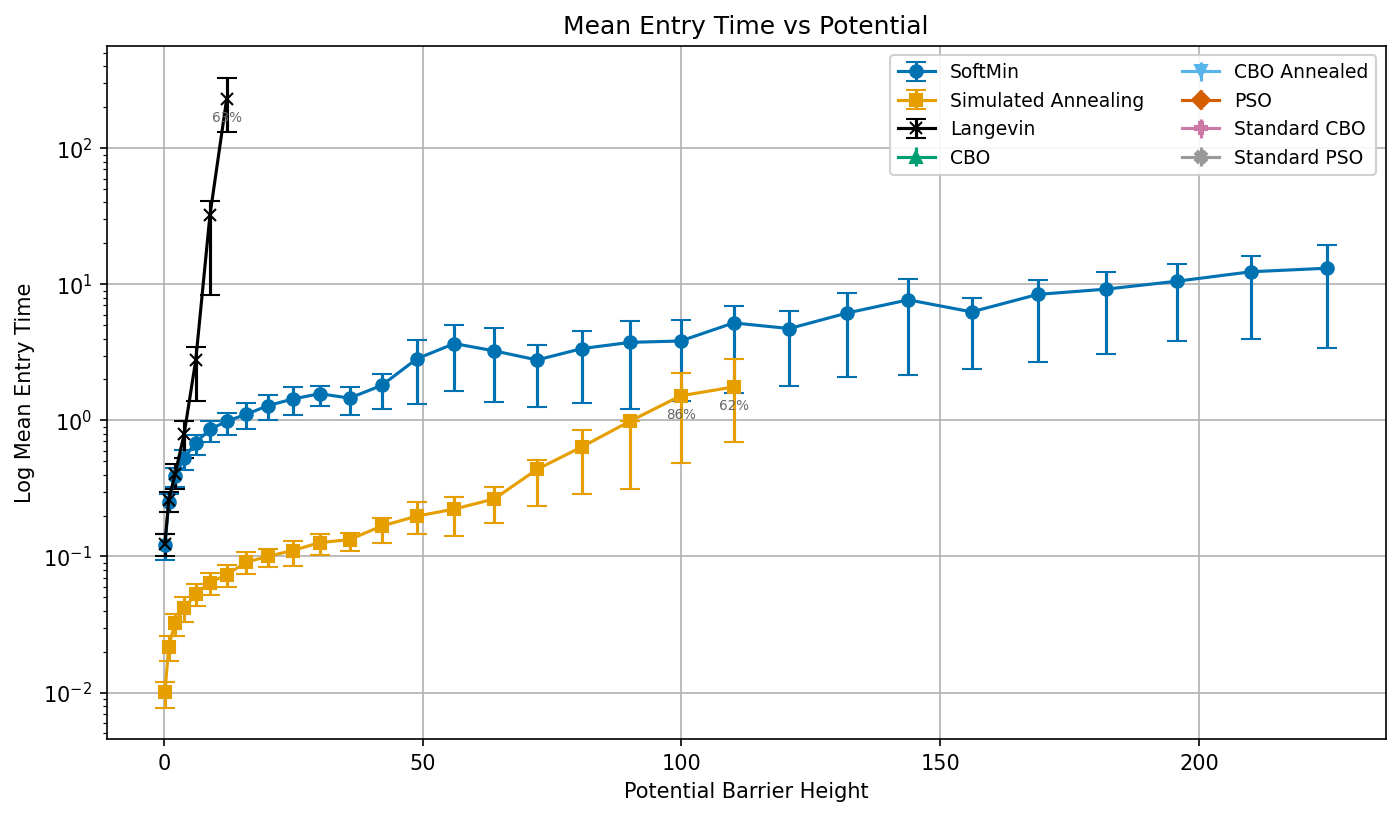
\includegraphics[width=\linewidth]{images/double_well_comparison.png}
  \end{minipage}\hfill
  \begin{minipage}{0.48\textwidth}
    \centering
    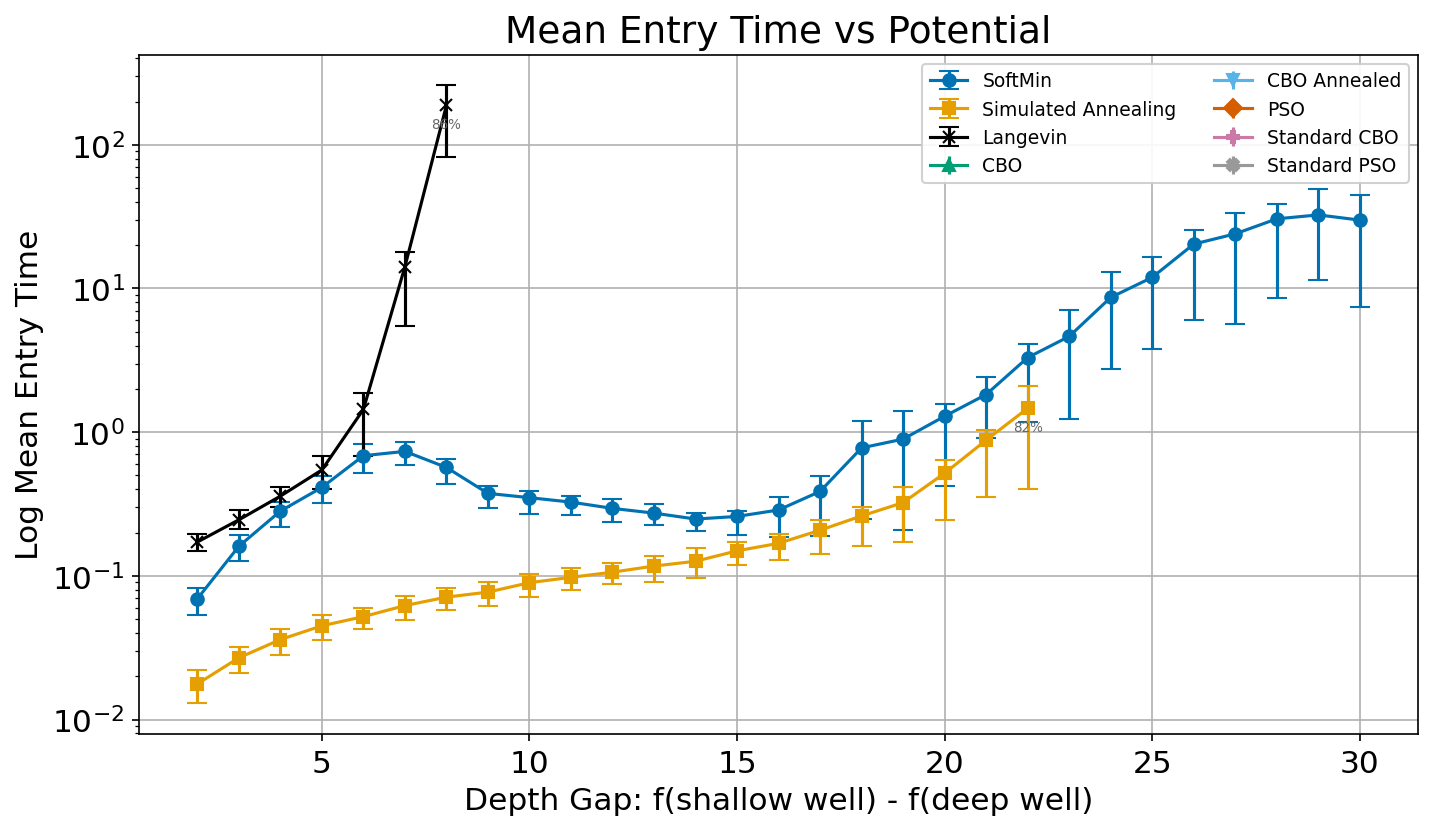
\includegraphics[width=\linewidth]{images/quadruple_well_comparison.png}
  \end{minipage}
  \caption{First-entry time into a value-space target, $\sigma=1$, in continuous-time units ($\text{steps}\times\eta$). Left: 1D double well vs.\ barrier height $h=f(s)-f(z_-)$. Right: 2D quadruple well vs.\ the depth gap between the shallow and deep wells, which equals $A$ exactly. Each point is the mean over seeds that reached the target, band spans their interquartile range; a point below a 50\% reached-fraction is omitted. CBO and PSO (gradient-aware and canonical alike) reach the target in at most 3\% of seeds at any swept difficulty on either benchmark and so never appear.}
  \label{fig:experiments}
\end{figure}

Softmin reaches the target at every difficulty tested on both benchmarks (100\% of seeds throughout), with entry time growing only mildly against exponentially growing barriers: e.g.\ a factor of about $110$ in entry time against a factor of about $1100$ in barrier height on the double well. Simulated Annealing is faster wherever it still succeeds, but its reliability collapses as the barrier grows (from 100\% to 0\% reached-fraction on both benchmarks); Langevin fails earlier still; CBO and PSO, gradient-aware and canonical alike, reach the target in at most 3\% of seeds at any difficulty tested and never appear. Softmin is therefore not the fastest method where Simulated Annealing still works, but is the only one that keeps working as the barrier grows. This trade-off is consistent with Simulated Annealing's calibrated cooling schedule: its initial temperature ($T_0\approx14$, well above Softmin's fixed $\sigma=1$) gives a single trajectory a much larger early noise budget than the ensemble's fixed-noise dynamics, letting it cross moderate barriers faster; the same schedule, however, cools to near zero after a fixed number of steps regardless of the barrier actually faced, so it freezes before larger barriers can be crossed (Appendix~\ref{app:hyperparameter-methodology}), which is exactly where its reliability collapses.

On Lennard-Jones clusters ($N\in\{13,38,55,75\}$ atoms, Cambridge Cluster Database \citep{wales1997global,jones1924determination}), Softmin's quenched-energy gap above the literature global minimum stays small and essentially flat (from $0$ at $N=13$ to $3.7$ at $N=75$) while every baseline's gap grows roughly linearly with $N$ (to $23$--$30$ at $N=75$); the advantage \emph{widens}, not narrows, with cluster size (figure in Appendix~\ref{apx:other-experiments}). The generalized Ackley function, by contrast, is the boundary case: Particle Swarm Optimization is fastest at every dimension $d\in\{10,\dots,90\}$ tested, by a wide margin, and Softmin does not reach the target below $d=30$. The sign-reversal mechanism is active throughout, since Ackley's barriers sit well above the switching level $r_c$, and Softmin's entry time and reliability both improve with $d$ exactly as those barriers shrink, consistent with, though not evidence for, Theorem~\ref{thm:barrier-cap-main}; but on a landscape whose difficulty is carried by the density of shallow minima rather than their depth, barrier flattening delivers reliability, not speed (full figures and discussion in Appendix~\ref{apx:other-experiments}).

\section{Conclusion}
\label{sec:conclusion}

We introduced a stochastic gradient-based particle swarm method driven by the Softmin energy $J_\beta$. The ensemble's running best value is always nonincreasing and, under a Polyak--\L{}ojasiewicz condition, converges at least as fast as ordinary gradient flow (Theorem~\ref{thm:ensemble-min}), for any temperature schedule; separately, the interaction caps the quasipotential barrier between adjacent basins at a level of order $1/\beta$, independently of the true barrier height (Theorem~\ref{thm:barrier-cap-main}). Experiments support these guarantees unevenly: the descent guarantee is borne out directly; the barrier cap is not the operative effect at the $\sigma=1$ noise level used for the benchmarks (an ablation, Appendix~\ref{apx:ablation-study}, finds the Gibbs weighting shared by all sign conventions the more likely source of the advantage there), but becomes decisive at lower temperature as the barrier grows, and the Ackley benchmark identifies a landscape, dominated by many shallow minima rather than deep barriers, on which barrier flattening alone is not sufficient for competitive speed. Sharpening the small-noise bound, extending it beyond $d=1$, and analyzing the mean-field limit as $n\to\infty$ are natural next steps; the full discussion of limitations and future work is in Appendix~\ref{apx:limitations}.

\bibliography{references}

\appendix

\section{Extended Related Work}
\label{apx:related-work}

\paragraph{Metaheuristic optimization methods}
Metaheuristic optimization methods include Consensus-Based Optimization (CBO) \citep{CarrilloChoiTotzeckTse2018,fornasier2024consensus,pinnau2017consensus, carrillo2021consensus}, Genetic Algorithms \citep{Goldberg1989}, Ant Colony Optimization \citep{DorigoStutzle2004}, and Particle Swarm Optimization (PSO) \citep{kennedy1995particle, noel2012new}. Traditional particle-swarm approaches typically operate without explicit gradient information, relying instead on position-based updates to coordinate particles toward promising regions. When reliable gradient information is available, leveraging it enables convergence rates comparable to standard stochastic gradient descent, which gradient-agnostic metaheuristics cannot achieve.

Recent gradient-based swarm methods \citep{riedl2023gradient, bolte2024swarm, carrillo2021consensus, noel2012new} have made progress by incorporating gradient information into multi-particle dynamics. However, our approach differs fundamentally in its mechanism for inducing exploration and escaping barriers. Rather than consensus-based averaging or general gradient-weighted potentials, we employ the Softmin energy functional to explicitly create a minimizing/maximizing partition of the particle ensemble: particles below the Softmin threshold are drawn toward local minima via gradient descent, while particles above the threshold are repelled toward maxima. This automatic role assignment (Theorem~\ref{thm:stationary-points}) simultaneously reduces effective potential barriers (Theorem~\ref{thm:transition-time}) and forces suboptimal particles into exploratory regimes without requiring manual basin-switching heuristics.

To the best of our knowledge, no other metaheuristic employs the Softmin energy functional, computed as the Softmin of function values at particle positions, as the sole source of inter-particle interaction. This design enables provable escape from suboptimal local minima with a barrier bounded independently of the true barrier height (Theorem~\ref{thm:transition-time}, Appendix~\ref{apx:barrier-full}), together with a deterministic guarantee that the ensemble's best value never lags ordinary gradient flow under a Polyak--\L{}ojasiewicz condition (Theorem~\ref{thm:ensemble-min}, Appendix~\ref{apx:technical-proofs}). Section~\ref{sec:numerical-experiments} tests these predictions on benchmark landscapes where barriers dominate the hardness, and reports both where the mechanism accounts for the observed performance and where it does not.

\paragraph{Langevin-based sampling and interacting-particle methods}
Stochastic Gradient Langevin Dynamics (SGLD) \citep{welling2011bayesian} and its non-asymptotic analysis for non-convex optimization \citep{raginsky2017nonconvex} study a single diffusion whose drift is the gradient of the objective itself, with guarantees governed by the spectral gap of the associated Gibbs measure; when multiple particles are used, interaction typically enters only through averaging over independent runs. Interacting Particle Langevin Dynamics (IPLD) \citep{akyildiz2025interacting, encinar2025proximal} instead couples an ensemble of particles through their empirical measure, using this mean-field interaction to build unbiased or stabilized estimators of the marginal likelihood gradient in latent-variable models. Our construction is closer in spirit to IPLD, in that it also relies on genuine ensemble-level coupling rather than independent copies, but the interaction itself is different in kind: instead of pooling particles through an empirical average, the Softmin energy $J_\beta$ couples particles through their relative energies, producing a state-dependent, sign-changing effective learning rate $\prefactor{k}{\xx}$ that deterministically assigns each particle a minimizing or maximizing role (Theorem~\ref{thm:stationary-points}). It is this competitive, temperature-sharpened coupling, rather than mean-field averaging, that produces the barrier-capping mechanism of Theorem~\ref{thm:transition-time}, and it is aimed directly at global optimization of $f$ rather than at marginal-likelihood estimation.

\paragraph{Connection to Statistical Physics and Functional Design}
Our approach shares conceptual roots with population-based statistical physics methods such as Population Annealing (PA) \citep{Wang_2015}, which also employs a Gibbs-weighted ensemble to locate global ground states. However, while PA relies on discrete demographic selection, duplicating low-energy particles and eliminating high-energy ones prior to local Markov Chain Monte Carlo steps, our method maintains a fixed population size and drives exploration through continuous dynamical repulsion. This active exploration mechanism differentiates our Softmin energy functional from the standard log-sum-exp (or free-energy) functional, $F_\beta(\xx) = -{\beta}^{-1} \log \sum e^{-\beta f(x_i)}$. The gradient of the log-sum-exp formulation, $\nabla_{x_k} F_\beta(\xx) = w_k \nabla f(x_k)$, strictly preserves gradient descent, causing sub-optimal particles with small weights to simply stagnate. In contrast, the gradient of our proposed Softmin functional, $J_\beta(\xx) = \sum w_i f(x_i)$, natively incorporates the sign-changing effective learning rate, $\prefactor{k}{\xx}$. Consequently, rather than discarding trapped particles, the geometry of the Softmin functional actively destabilizes their local minima, forcing high-energy particles to hill-climb and escape via the energy barrier-flattening mechanism formalized in our theoretical analysis.

\paragraph{Softmin energy} Theoretical work on the Gibbs Softmin (or Boltzmann Softmin) has primarily focused on its properties as a smooth approximation to the minimum operator \citep{bertsekas1999nonlinear}, convergence of softmax policy gradients in reinforcement learning \citep{mei2020global}, and its role in exploration-exploitation trade-offs via temperature scheduling \citep{song2019revisiting}. To our knowledge, this is the first work employing $J_\beta$ as an optimization objective for non-convex global search. This is conceptually distinct from swarm-gradient methods that anneal a mean-field particle density toward the Dirac mass at the global minimizer \citep{bolte2024swarm}: rather than acting on a population density, the Softmin energy couples particles directly through the relative ranking of their objective values. The effective barrier reduction via particle cooperation, analyzed in Theorem~\ref{thm:transition-time}, is previously unstudied.

\section{Freidlin--Wentzell Large Deviation Theory}
\label{apx:fw-theory}

This appendix summarizes the background large deviation theory used by Theorem~\ref{thm:transition-time} and Corollary~\ref{cor:exit-time-conditional}. Consider a small-noise gradient diffusion on $\R^N$,
\[
    \dd\XX_t = -\nabla U(\XX_t)\dd t + \sqrt{2\sigma}\dd B_t,
\]
for a potential $U\in C^2(\R^N)$ and standard $N$-dimensional Brownian motion $(B_t)_{t\ge0}$; in our application $N=nd$ and $U=nJ_\beta$. As $\sigma\downarrow0$, sample paths of this diffusion concentrate around trajectories of the noiseless flow $\dot\XX_t=-\nabla U(\XX_t)$, and rare deviations from this flow are governed by the Freidlin--Wentzell large deviation principle \citep{freidlin2012random}. For an absolutely continuous path $\phi:[0,T]\to\R^N$, the Freidlin--Wentzell action is
\begin{equation}
    I_{0T}(\phi):=\frac14\int_0^T\bigl\|\dot\phi(t)+\nabla U(\phi(t))\bigr\|^2\dd t,
    \label{eq:fw-action}
\end{equation}
and the quasipotential between a point $x\in\R^N$ and a closed set $A\subset\R^N$ is
\begin{equation}
    V(x,A):=\inf_{T>0}\ \inf_{\substack{\phi(0)=x\\ \phi(T)\in A}}I_{0T}(\phi).
    \label{eq:fw-quasipotential}
\end{equation}
Intuitively, $I_{0T}(\phi)$ penalizes deviation from the noiseless flow, vanishing exactly along trajectories of $\dot\phi=-\nabla U(\phi)$; $V(x,A)$ is the cheapest such penalty over all paths from $x$ reaching $A$, and quantifies how atypical (large-deviation-improbable) it is for the diffusion to travel from $x$ to $A$ without the help of noise. The infimum in \eqref{eq:fw-quasipotential} need not be attained by any single finite-time path: it is generally only approximated arbitrarily well, e.g.\ by following the time-reversed noiseless flow toward $x$ and then the forward flow toward $A$, taking arbitrarily long to approach the relevant critical points. This is the sense in which quasipotential values are computed exactly, rather than merely bounded, in the proof of Theorem~\ref{thm:transition-time} below.

Under the standard hypotheses of Freidlin--Wentzell exit theory \citep{freidlin2012random} (in particular that $D$ is a bounded domain with $x\in D$, that $x$ is the unique asymptotically stable equilibrium of the noiseless flow in $D$, and that $\partial D$ contains no other equilibria), the exit time $\tau_D^\sigma$ of the diffusion from $D$, started at $x$, satisfies
\begin{equation}
    \lim_{\sigma\downarrow0}\sigma\log \E_x\tau_D^\sigma = V(x,\partial D).
    \label{eq:fw-exit-theorem}
\end{equation}

For a gradient drift, the action of any path admits the exact decomposition
\begin{equation}
    I_{0T}(\phi) = U(\phi(T))-U(\phi(0)) + \frac14\int_0^T\bigl\|\dot\phi(t)-\nabla U(\phi(t))\bigr\|^2\dd t,
    \label{eq:gradient-decomposition}
\end{equation}
obtained by expanding the square in \eqref{eq:fw-action} and completing it against $\dd U(\phi(t))/\dd t = \langle\nabla U(\phi(t)),\dot\phi(t)\rangle$. Consequently, any segment of $\phi$ that follows the noiseless flow \emph{downhill} (i.e.\ $\dot\phi=-\nabla U(\phi)$) contributes zero action, while a segment moving \emph{uphill} against the flow (i.e.\ $\dot\phi=\nabla U(\phi)$) costs exactly the potential increase along that segment. This identity is what allows the quasipotential of an explicit admissible path to be computed exactly, rather than merely bounded, in the proof of Theorem~\ref{thm:transition-time}.

\section{Technical Proofs}
\label{apx:technical-proofs}

\subsection{Proofs for Section~\ref{sec:method}}

\begin{lemma}[Component gradient and Hessian at critical configurations]
    \label{lem:derivative-of-J-proof}
    Let $w_k = e^{-\beta f(x_k)}(\sum_j e^{-\beta f(x_j)})^{-1}$ denote the Gibbs weight of particle $x_k$, and let $\prefactor{k}{\xx} = nw_k\left[1 - \beta(f(x_k) - J_\beta(\xx))\right]$ be the dynamic pre-factor. Then
    \begin{equation}
        \nabla_{x_k} (nJ_\beta(\xx)) = \prefactor{k}{\xx} \nabla f(x_k),
        \qquad
        \sum_{k=1}^n \prefactor{k}{\xx} = n.
        \label{eq:lemma-gradient}
    \end{equation}
    Moreover, for $k \neq \ell$ the mixed Hessian block is the outer product
    \begin{equation}
        \frac{\partial^2 (nJ_\beta(\xx))}{\partial x_\ell \partial x_k} = \nabla f(x_k)\bigl(\nabla_{x_\ell}\prefactor{k}{\xx}\bigr)^\top,
        \label{eq:mixed-block}
    \end{equation}
    which vanishes whenever $\nabla f(x_k)=0$. Consequently, if $\xx$ is such that $\nabla f(x_k)=0$ for every $k$, then $\nabla(nJ_\beta(\xx))=0$ and the Hessian is block diagonal,
    \begin{equation}
        \nabla^2(nJ_\beta(\xx)) = \operatorname{blockdiag}\bigl(\prefactor{1}{\xx}\nabla^2 f(x_1),\dots,\prefactor{n}{\xx}\nabla^2 f(x_n)\bigr).
        \label{eq:block-diagonal-hessian}
    \end{equation}
    Finally, if $\prefactor{k}{\xx}=0$ then $\frac{\partial^2(nJ_\beta(\xx))}{\partial x_k^2} = -n\beta w_k \nabla f(x_k)\nabla f(x_k)^\top$.
\end{lemma}

\begin{proof}
    We compute the derivatives using the chain rule and the properties of the Gibbs weights. First, we establish the gradient of the weight $w_i$ with respect to $x_k$:
    \begin{equation*}
        \nabla_{x_k} w_i = \begin{cases}
            \beta w_i w_k \nabla f(x_k) & \text{if } i \neq k, \\
            -\beta w_k (1 - w_k) \nabla f(x_k) & \text{if } i = k.
        \end{cases}
    \end{equation*}
    For the first derivative of $nJ_\beta(\xx) = n\sum_i w_i f(x_i)$, an identical computation to the main text gives $\nabla_{x_k}(nJ_\beta(\xx)) = nw_k[1-\beta(f(x_k)-J_\beta(\xx))]\nabla f(x_k) = \prefactor{k}{\xx}\nabla f(x_k)$; summing over $k$ and using $\sum_k w_k=1$, $\sum_k w_kf(x_k)=J_\beta(\xx)$, gives $\sum_k\prefactor{k}{\xx}=n[1-\beta(J_\beta(\xx)-J_\beta(\xx))]=n$.

    For the mixed second derivative ($k\ne\ell$), we differentiate $\nabla_{x_k}(nJ_\beta(\xx))=\prefactor{k}{\xx}\nabla f(x_k)$ with respect to $x_\ell$. Because $\nabla f(x_k)$ is independent of $x_\ell$, the Jacobian matrix is the outer product $\nabla f(x_k)(\nabla_{x_\ell}\prefactor{k}{\xx})^\top$. Substituting $\nabla_{x_\ell}w_k=\beta w_kw_\ell\nabla f(x_\ell)$ and $\nabla_{x_\ell}J_\beta(\xx)=\frac1n\prefactor{\ell}{\xx}\nabla f(x_\ell)$,
    \begin{align*}
        \nabla_{x_\ell}\prefactor{k}{\xx} &= n(\nabla_{x_\ell}w_k)\left[1-\beta(f(x_k)-J_\beta(\xx))\right] + nw_k\beta\left(\nabla_{x_\ell}J_\beta(\xx)\right) \\
        &= \beta w_\ell\bigl(nw_k[1-\beta(f(x_k)-J_\beta(\xx))]\bigr)\nabla f(x_\ell) + \beta w_k\prefactor{\ell}{\xx}\nabla f(x_\ell) \\
        &= \beta\left[w_\ell\prefactor{k}{\xx}+w_k\prefactor{\ell}{\xx}\right]\nabla f(x_\ell),
    \end{align*}
    which gives \eqref{eq:mixed-block} and vanishes whenever $\nabla f(x_k)=0$ (or symmetrically $\nabla f(x_\ell)=0$). If $\nabla f(x_k)=0$ for every $k$, every off-diagonal block vanishes and \eqref{eq:lemma-gradient} gives $\nabla(nJ_\beta(\xx))=0$; the diagonal block computed below then reduces to $\prefactor{k}{\xx}\nabla^2f(x_k)$, giving the block-diagonal form \eqref{eq:block-diagonal-hessian}.

    Finally, for the diagonal block ($k=\ell$), applying the product rule to $\nabla_{x_k}(nJ_\beta(\xx))=\prefactor{k}{\xx}\nabla f(x_k)$ includes the local Hessian $\nabla^2 f(x_k)$:
    \[
        \frac{\partial^2(nJ_\beta(\xx))}{\partial x_k^2} = \prefactor{k}{\xx}\nabla^2f(x_k) + \nabla f(x_k)\bigl(\nabla_{x_k}\prefactor{k}{\xx}\bigr)^\top.
    \]
    Using $\nabla_{x_k}w_k=-\beta w_k(1-w_k)\nabla f(x_k)$ and $\nabla_{x_k}J_\beta(\xx)=\frac1n\prefactor{k}{\xx}\nabla f(x_k)$, a computation identical in structure to the mixed case gives
    \[
        \nabla_{x_k}\prefactor{k}{\xx} = -\beta\left[nw_k+\prefactor{k}{\xx}-2w_k\prefactor{k}{\xx}\right]\nabla f(x_k),
    \]
    so that, substituting back,
    \[
        \frac{\partial^2(nJ_\beta(\xx))}{\partial x_k^2} = \prefactor{k}{\xx}\nabla^2f(x_k) - \beta\left[nw_k+\prefactor{k}{\xx}-2w_k\prefactor{k}{\xx}\right]\nabla f(x_k)\nabla f(x_k)^\top,
    \]
    which reduces to $-n\beta w_k\nabla f(x_k)\nabla f(x_k)^\top$ when $\prefactor{k}{\xx}=0$. \qedhere
\end{proof}

\begin{proof}[Proof of Theorem~\ref{thm:stationary-points}]
    A locally asymptotically stable equilibrium of the gradient flow is an isolated local minimum of $nJ_\beta$: indeed $\frac{d}{dt}(nJ_\beta(\xx(t)))=-\|\nabla(nJ_\beta)\|^2\le0$, so if points arbitrarily close to $\bar\xx$ had strictly smaller value the trajectories starting there could not converge to $\bar\xx$; and a non-isolated equilibrium admits nearby constant trajectories that likewise do not converge to $\bar\xx$.

    Fix $k$ and freeze the other particles at $\bar x_j$, $j\ne k$. Since $nJ_\beta$ depends on $x_k$ only through $r=f(x_k)$, we may write
    \[
        nJ_\beta(\bar x_1,\dots,x_k,\dots,\bar x_n)=g(f(x_k)), \qquad g(r):=n\,\frac{re^{-\beta r}+C_1}{e^{-\beta r}+C_0},
    \]
    with $C_0:=\sum_{j\ne k}e^{-\beta f(\bar x_j)}>0$ and $C_1:=\sum_{j\ne k}f(\bar x_j)e^{-\beta f(\bar x_j)}$. By the chain rule and Lemma~\ref{lem:derivative-of-J-proof}, wherever $\nabla f(x_k)\ne0$ one has $g'(f(x_k))=\prefactor{k}{\xx}$; by continuity of both sides in $f(x_k)$, $g'(f(\bar x_k))=\prefactor{k}{\bar\xx}$. Writing $g'(r)=n\omega(r)[1-\beta(r-g(r)/n)]$ with $\omega(r)=e^{-\beta r}/(e^{-\beta r}+C_0)\in(0,1)$, a direct computation shows that at any critical point $r_0$ of $g$ (where the bracket vanishes), $g''(r_0)=-n\beta\omega(r_0)<0$.

    \emph{Step 1: $\prefactor{k}{\bar\xx}\ne0$.} Suppose $\prefactor{k}{\bar\xx}=0$. By the above, $r_0=f(\bar x_k)$ is a critical point of $g$, and it is a strict local maximum. If $f$ is non-constant near $\bar x_k$, there are points $y$ arbitrarily close to $\bar x_k$ with $f(y)$ close to but different from $r_0$, whence $nJ_\beta(\dots,y,\dots)=g(f(y))<g(r_0)=nJ_\beta(\bar\xx)$, contradicting local minimality. If $f$ is constant near $\bar x_k$, moving $x_k$ within that level set leaves every objective value, Gibbs weight, and gradient unchanged, producing a continuum of equilibria arbitrarily close to $\bar\xx$ and contradicting isolation. Hence $\prefactor{k}{\bar\xx}\ne0$.

    \emph{Step 2: $\nabla f(\bar x_k)=0$.} Since $\prefactor{k}{\bar\xx}\ne0$, $g'(f(\bar x_k))\ne0$, so $g$ is strictly monotone near $f(\bar x_k)$. If $\nabla f(\bar x_k)\ne0$, then $f$ takes values on both sides of $f(\bar x_k)$ arbitrarily near $\bar x_k$; strict monotonicity of $g$ then yields nearby configurations with $nJ_\beta<nJ_\beta(\bar\xx)$, contradicting local minimality. Hence $\nabla f(\bar x_k)=0$.

    \emph{Step 3: classification.} If $\prefactor{k}{\bar\xx}>0$, then $g$ is strictly increasing near $f(\bar x_k)$, so local minimality of $nJ_\beta$ forces $f(x_k)\ge f(\bar x_k)$ for $x_k$ near $\bar x_k$; thus $\bar x_k$ is a local minimum of $f$. If $\prefactor{k}{\bar\xx}<0$, the symmetric argument shows $\bar x_k$ is a local maximum. Because $nw_k>0$, the sign of $\prefactor{k}{\bar\xx}$ is that of $1-\beta(f(\bar x_k)-J_\beta(\bar\xx))$, giving the stated threshold. Finally, $\sum_k\prefactor{k}{\bar\xx}=n$ forces some $\prefactor{k}{\bar\xx}>0$, so at least one particle is at a local minimum of $f$.
\end{proof}

\begin{corollary}[Sufficient condition for stability]
\label{cor:stability-sufficient}
Let $\bar\xx=(\bar x_1,\dots,\bar x_n)$ satisfy $\nabla f(\bar x_k)=0$ for every $k$, and assume that for each $k$ either
\[
    \prefactor{k}{\bar\xx}>0 \text{ and } \nabla^2f(\bar x_k)\succ0,
    \qquad\text{or}\qquad
    \prefactor{k}{\bar\xx}<0 \text{ and } \nabla^2f(\bar x_k)\prec0,
\]
evaluated at $\bar\xx$. Then $\nabla^2(nJ_\beta)(\bar\xx)\succ0$; in particular $\bar\xx$ is a strict local minimum of $nJ_\beta$ and a locally asymptotically stable equilibrium of the gradient flow.
\end{corollary}

\begin{proof}
    By Lemma~\ref{lem:derivative-of-J-proof} the Hessian at a fully critical configuration is block diagonal with blocks $\prefactor{k}{\bar\xx}\nabla^2f(\bar x_k)$, and each hypothesis makes the corresponding block positive definite.
\end{proof}

\begin{remark}[Global existence]
    \label{rem:global-existence}
    Theorem~\ref{thm:ensemble-min} presupposes a global solution. Since $m$ is nonincreasing, every particle attaining the running minimum stays in the compact sublevel set $S_0$ when $f$ is coercive; the theorem controls these particles only. Maximizing particles ($\prefactor{k}{\xx(t)}<0$) are not controlled by this estimate, but they are damped strongly enough that blow-up is easy to exclude. Write $u_k(t):=f(x_k(t))-m(t)\ge0$. From $\sum_je^{-\beta_tf(x_j)}\ge e^{-\beta_tm}$ we get $w_k\le e^{-\beta_tu_k}$, and hence $\beta_t\bigl(J_{\beta_t}(\xx)-m\bigr)=\beta_t\sum_jw_ju_j\le\beta_t\sum_ju_je^{-\beta_tu_j}\le n/e$. Therefore
    \[
        |\prefactor{k}{\xx(t)}|\;\le\; n\bigl(1+\beta_tu_k+n/e\bigr)e^{-\beta_tu_k}\;\le\;n\bigl(1+n/e\bigr),
    \]
    using $(1+v)e^{-v}\le1$ and $e^{-v}\le1$ for $v\ge0$. The pre-factor is thus bounded uniformly and decays exponentially in the particle's energy gap, so for coercive $f$ whose gradient grows at most polynomially in $f$ the drift stays bounded along trajectories and global solutions exist. We nonetheless state the theorem for a given global solution, since its conclusion concerns only the minimizing particles.
\end{remark}

\begin{proof}[Proof of Theorem~\ref{thm:ensemble-min}]
    Fix $t$ and let $i$ attain the minimum, $f(x_i(t))=m(t)$. Since $f(x_i(t))\le f(x_j(t))$ for all $j$, we have $e^{-\beta_tf(x_j(t))}\le e^{-\beta_tf(x_i(t))}$, hence $\sum_je^{-\beta_tf(x_j(t))}\le ne^{-\beta_tf(x_i(t))}$ and therefore $nw_i(t)\ge1$. As $J_{\beta_t}(\xx(t))$ is a convex combination of the values $f(x_j(t))$, it satisfies $J_{\beta_t}(\xx(t))\ge f(x_i(t))$, so $1-\beta_t(f(x_i(t))-J_{\beta_t}(\xx(t)))\ge1$. Multiplying,
    \begin{equation}
        \prefactor{i}{\xx(t)}\ge1 \qquad \text{for every } i \text{ attaining the minimum at } t.
        \label{eq:ai-ge-1}
    \end{equation}
    Along such a particle,
    \[
        \frac{d}{dt}f(x_i(t)) = \langle\nabla f(x_i(t)),\dot x_i(t)\rangle = -\prefactor{i}{\xx(t)}\|\nabla f(x_i(t))\|^2 \le -\|\nabla f(x_i(t))\|^2.
    \]

    Consider $m=\min_k g_k$ with $g_k(t)=f(x_k(t))$. Since $\beta_t$ is only assumed measurable, each $x_k$ is a Carath\'eodory solution and hence absolutely continuous; as $f$ has locally Lipschitz gradient, each $g_k$ is absolutely continuous on compact time intervals, and a pointwise minimum of finitely many absolutely continuous functions is absolutely continuous. Therefore $m$ is absolutely continuous, and $m$ together with every $g_k$ is differentiable at a.e.\ $t$. At any such $t$, choose $i$ attaining the minimum; the function $g_i-m\ge0$ is then differentiable at $t$ and vanishes there, so it has zero derivative at $t$, giving $m'(t)=g_i'(t)$. Combined with the previous display,
    \[
        m'(t)=-\prefactor{i}{\xx(t)}\|\nabla f(x_i(t))\|^2\le-\|\nabla f(x_i(t))\|^2\le0 \qquad \text{for a.e. } t.
    \]
    Integrating, $m$ is nonincreasing, so every minimizing particle stays in $S_0=\{x:f(x)\le m(0)\}$, where the Polyak--\L{}ojasiewicz condition (Definition~\ref{def:pl-condition}) applies:
    \[
        m'(t)\le-\|\nabla f(x_i(t))\|^2\le-2\mu\bigl(f(x_i(t))-f_\star\bigr)=-2\mu\bigl(m(t)-f_\star\bigr).
    \]
    Setting $y(t):=e^{2\mu t}(m(t)-f_\star)$, which is absolutely continuous, we get $y'(t)=e^{2\mu t}[m'(t)+2\mu(m(t)-f_\star)]\le0$ for a.e.\ $t$, so $y(t)\le y(0)$, i.e.
    \[
        m(t)-f_\star\le e^{-2\mu t}\bigl(m(0)-f_\star\bigr), \qquad t\ge0. \qedhere
    \]
\end{proof}

\subsection{Barrier flattening: full statement and proofs}
\label{apx:barrier-full}

This appendix gives the full, three-part version of Theorem~\ref{thm:barrier-cap-main} and its proof. Fix $n\ge2$, $\beta>0$, and $d=1$. Consider three consecutive nondegenerate critical points of $f$,
\[
    z_-<s<z_+,
\]
with $z_\pm$ local minima and $s$ the separating local maximum, and assume
\begin{equation}
    f'(x)>0 \text{ on } (z_-,s), \qquad f'(x)<0 \text{ on } (s,z_+).
    \label{eq:adjacent-well-monotonicity}
\end{equation}
Set the relative energy and the barrier height
\begin{equation}
    r(x):=f(x)-f(z_-), \qquad h:=r(s)>0, \qquad \rho_+:=r(z_+)<h.
    \label{eq:relative-energy}
\end{equation}
The case of interest is $\rho_+<0$, in which $z_+$ is a strictly deeper minimum than $z_-$.

\begin{assumption}
\label{assum:channel}
$f\in C^2(\R)$; $z_-<s<z_+$ are nondegenerate critical points of $f$ (i.e.\ $f''(z_-)>0$, $f''(s)<0$, $f''(z_+)>0$) satisfying the monotonicity condition \eqref{eq:adjacent-well-monotonicity}; and $n\ge2$, $\beta>0$, $d=1$.
\end{assumption}

\begin{remark}[Metastability of the initial state]
\label{rem:metastable-init}
At the consensus configuration $\bar\xx=(z_-,\dots,z_-)$, every Gibbs weight equals $1/n$, so $\prefactor{k}{\bar\xx}\equiv1$ for every $k$. By Corollary~\ref{cor:stability-sufficient}, using $f''(z_-)>0$, $\bar\xx$ is therefore a strict local minimum of $nJ_\beta$ and a locally asymptotically stable equilibrium of the gradient flow, i.e.\ genuinely metastable for the noisy dynamics at small $\sigma$.
\end{remark}

We rely on the Freidlin--Wentzell large deviation theory for exit times of small-noise diffusions from metastable domains, summarized in Appendix~\ref{apx:fw-theory}: under the standard hypotheses of that theory, the exit time $\tau_D^\sigma$ from a metastable domain $D$ satisfies $\lim_{\sigma\downarrow0}\sigma\log \E_{\xx}\tau_D^\sigma=V_\beta(\xx,\partial D)$, where $V_\beta$ is the Freidlin--Wentzell quasipotential associated with the noisy dynamics at fixed $\beta$.

To build an admissible escape path, freeze $n-1$ particles at $z_-$ and let one particle move:
\begin{equation}
    \Gamma(x):=(x,z_-,\dots,z_-).
    \label{eq:channel}
\end{equation}
Factoring $e^{-\beta f(z_-)}$ out of the Gibbs weights gives $J_\beta(\Gamma(x))=f(z_-)+u(r(x))/n$, that is, the exact identity
\begin{equation}
    nJ_\beta(\Gamma(x))=nf(z_-)+u(r(x)), \qquad u(r):=\frac{n\,r\,e^{-\beta r}}{\,n-1+e^{-\beta r}\,}, \quad r\in\R,
    \label{eq:reduced-potential}
\end{equation}
where $u$ is the \emph{reduced potential}. The additive constant $nf(z_-)$ does not enter $\nabla(nJ_\beta)$, and both the action and the quasipotential depend on $nJ_\beta$ only through its increments.

\begin{lemma}[Channel invariance and reduced gradient flow]
\label{lem:channel-invariant}
The set $\{\Gamma(x):x\in\R\}$ is invariant under the noiseless gradient flow, since $f'(z_-)=0$ forces the frozen coordinates' drift to vanish identically. On this invariant manifold, the dynamics reduces to the one-dimensional gradient flow $\dot x=-W'(x)$ of the reduced potential $W(x):=u(r(x))$ of \eqref{eq:reduced-potential}.
\end{lemma}

\begin{proof}
Since $z_-$ is a critical point of $f$, every frozen coordinate satisfies $\dot x_j=-\prefactor{j}{\Gamma(x)}f'(z_-)=0$, so $\{\Gamma(x):x\in\R\}$ is invariant. Differentiating \eqref{eq:reduced-potential} along the channel gives $W'(x)=\frac{d}{dx}\bigl[nJ_\beta(\Gamma(x))\bigr]=u'(r(x))r'(x)=u'(r(x))f'(x)$; applying the chain rule directly to $nJ_\beta$ and \eqref{eq:softmin-gradient} gives the same derivative as $\prefactor{1}{\Gamma(x)}f'(x)$. Hence $W'(x)=\prefactor{1}{\Gamma(x)}f'(x)$, matching the active coordinate's drift $-\prefactor{1}{\Gamma(x)}f'(x)$, and in particular reproving $\prefactor{1}{\Gamma(x)}=u'(r(x))$, made explicit in closed form in Lemma~\ref{lem:channel-drift} below.
\end{proof}

\begin{lemma}[Channel drift and shape of the reduced potential]
\label{lem:channel-drift}
Let $\prefactor{1}{\Gamma(x)}$ denote the pre-factor of the active particle along the channel. Then, for every $x\in\R$,
\begin{equation}
    \prefactor{1}{\Gamma(x)}=u'(r(x))
    =\frac{n\,e^{-\beta r(x)}\,q(r(x))}{\bigl(n-1+e^{-\beta r(x)}\bigr)^{2}},
    \qquad
    q(r):=(n-1)(1-\beta r)+e^{-\beta r}.
    \label{eq:a1-equals-uprime}
\end{equation}
The function $q$ is strictly decreasing on $\R$ and has a unique zero $r_c$, which satisfies
\begin{equation}
    \frac1\beta<r_c<\frac{n}{(n-1)\beta}.
    \label{eq:rc-location}
\end{equation}
Consequently $u$ is strictly increasing on $(-\infty,r_c]$ and strictly decreasing on $[r_c,\infty)$, and $r_c$ is exactly the relative-energy level at which the active particle switches from minimizing to maximizing, i.e.\ the level at which $f(x)-J_\beta(\Gamma(x))=1/\beta$.
\end{lemma}

\begin{proof}
    Write $r:=r(x)$. Factoring $e^{-\beta f(z_-)}$ out of the Gibbs weights at $\Gamma(x)$,
    \[
        w_1(\Gamma(x))=\frac{e^{-\beta r}}{n-1+e^{-\beta r}}, \qquad w_j(\Gamma(x))=\frac{1}{n-1+e^{-\beta r}} \quad (j\ge2),
    \]
    whence $J_\beta(\Gamma(x))-f(z_-)=re^{-\beta r}/(n-1+e^{-\beta r})=u(r)/n$, which is \eqref{eq:reduced-potential}. Therefore
    \[
        f(x)-J_\beta(\Gamma(x)) = r-\frac{re^{-\beta r}}{n-1+e^{-\beta r}} = \frac{(n-1)r}{n-1+e^{-\beta r}},
    \]
    and substituting into $\prefactor{1}{\Gamma(x)}=nw_1(\Gamma(x))[1-\beta(f(x)-J_\beta(\Gamma(x)))]$ gives
    \[
        \prefactor{1}{\Gamma(x)} = \frac{ne^{-\beta r}}{n-1+e^{-\beta r}}\cdot\frac{n-1+e^{-\beta r}-\beta(n-1)r}{n-1+e^{-\beta r}} = \frac{ne^{-\beta r}q(r)}{(n-1+e^{-\beta r})^2}.
    \]
    Differentiating \eqref{eq:reduced-potential} directly yields the same expression for $u'(r)$, proving \eqref{eq:a1-equals-uprime}, consistently with the identity $\prefactor{1}{\Gamma(x)}=u'(r(x))$ already established in Lemma~\ref{lem:channel-invariant}. In particular $\prefactor{1}{\Gamma(x)}=0$ if and only if $q(r)=0$, which by the displayed formula for $f(x)-J_\beta$ is equivalent to $f(x)-J_\beta(\Gamma(x))=1/\beta$, i.e.\ to the vanishing of the Softmin threshold gap of the active particle.

    Since $q'(r)=-\beta(n-1)-\beta e^{-\beta r}<0$ for all $r\in\R$, $q(0)=n>0$, and $q(r)\to-\infty$ as $r\to\infty$, $q$ has a unique zero $r_c>0$. From $q(1/\beta)=e^{-1}>0$ we get $r_c>1/\beta$; and $q(r_c)=0$ reads $(n-1)(\beta r_c-1)=e^{-\beta r_c}<1$, giving $\beta r_c<n/(n-1)$. This is \eqref{eq:rc-location}. As $ne^{-\beta r}/(n-1+e^{-\beta r})^2>0$, the sign of $u'$ is the sign of $q$, so $u$ is strictly increasing on $(-\infty,r_c]$ and strictly decreasing on $[r_c,\infty)$.
\end{proof}

We abbreviate the two relevant channel heights by
\begin{equation}
    u_c:=u(r_c)=\max_{r\in\R}u(r),
    \qquad
    u_h:=\max_{0\le r\le h}u(r)=u\bigl(\min\{h,r_c\}\bigr).
    \label{eq:channel-heights}
\end{equation}

\begin{theorem}[One-dimensional basin exit and post-saddle passage]
\label{thm:transition-time}
Under Assumption~\ref{assum:channel}, the following hold.
\begin{enumerate}
    \item \textbf{(Uniform barrier cap.)}
    \begin{equation}
        u_c=\max_{r\in\R}u(r)<\frac{n}{e(n-1)\beta}.
        \label{eq:barrier-cap-appendix}
    \end{equation}
    Both $u_c$ and, by \eqref{eq:rc-location}, $r_c$ are of order $\beta^{-1}$, uniformly in $h$.

    \item \textbf{(Initial basin exit: quasipotential bound.)}
    The infimum of the action among channel paths joining $\Gamma(z_-)$ to $\Gamma(s)$ equals $u_h$. Consequently
    \begin{equation}
        V_\beta\bigl(\Gamma(z_-),\Gamma(s)\bigr)\le u_h<\min\{h,r_c\}\le h.
        \label{eq:initial-bound}
    \end{equation}

    \item \textbf{(Post-saddle well and passage.)}
    Assume
    \begin{equation}
        r_c<h.
        \label{eq:high-barrier-regime}
    \end{equation}
    Then $\Gamma(s)$ is a strict local minimum of $nJ_\beta$, with channel barrier $u_c-u(h)$ on the $z_-$ side. On the $z_+$ side:
    \begin{itemize}
        \item If $\rho_+<r_c$, there is a unique $\xi_+\in(s,z_+)$ with $r(\xi_+)=r_c$, the channel well at $\Gamma(s)$ has matching barrier height $u_c-u(h)$ on this side, and
        \begin{equation}
            V_\beta\bigl(\Gamma(s),\Gamma(\xi_+)\bigr)\le u_c-u(h)<u_c;
            \label{eq:post-saddle-bound}
        \end{equation}
        \item If instead $\rho_+\ge r_c$, no point $\xi_+$ exists and the channel potential rises monotonically from $\Gamma(s)$ to $\Gamma(z_+)$, so no intermediate barrier separates them, with total rise $u(\rho_+)-u(h)\le u_c-u(h)$.
    \end{itemize}
    When $\rho_+<r_c$, concatenating the two crossings gives
    \begin{equation}
        V_\beta\bigl(\Gamma(z_-),\Gamma(\xi_+)\bigr) \;\le\; u_h+\bigl(u_c-u(h)\bigr) \;\le\; 2u_c-u(h) \;<\; \frac{2n}{e(n-1)\beta},
        \label{eq:two-stage-bound}
    \end{equation}
    by \eqref{eq:initial-bound}, \eqref{eq:post-saddle-bound}, and $u_h\le u_c$. Under the standing hypothesis $r_c<h$ of this part one has $u_h=u_c$, so the second inequality in \eqref{eq:two-stage-bound} is in fact an equality.
    If instead $h\le r_c$, $\Gamma(s)$ is not a local minimum of $nJ_\beta$ and no post-saddle well forms.
\end{enumerate}
\end{theorem}

\begin{proof}
    \emph{Part 1.} For $r\le0$ we have $u(r)\le0$. For $r>0$, since $n-1+e^{-\beta r}>n-1$,
    \[
        u(r)<\frac{n}{n-1}re^{-\beta r}\le\frac{n}{n-1}\max_{\rho\ge0}\rho e^{-\beta\rho}=\frac{n}{e(n-1)\beta},
    \]
    the maximum being attained at $\rho=1/\beta$. Hence $u_c=\max_\R u<n/(e(n-1)\beta)$, which is \eqref{eq:barrier-cap-appendix}; the bound on $r_c$ is \eqref{eq:rc-location}.

    \emph{Part 2.} A channel path has the form $\phi(t)=\Gamma(\psi(t))$; the frozen coordinates stay at the critical point $z_-$, so their drift vanishes and, with $W(x):=u(r(x))$, the action reduces to $I_{0T}=\frac14\int_0^T|\dot\psi+W'(\psi)|^2\dd t$. The one-dimensional version of \eqref{eq:gradient-decomposition} is
    \[
        I_{0T}=W(\psi(T))-W(\psi(0))+\frac14\int_0^T|\dot\psi-W'(\psi)|^2\dd t.
    \]
    By \eqref{eq:adjacent-well-monotonicity}, $r$ is a strictly increasing bijection from $[z_-,s]$ onto $[0,h]$, so there is a unique $x_m\in(z_-,s]$ with $r(x_m)=\min\{h,r_c\}$. On $[z_-,x_m]$ we have $r(x)\le r_c$, so by Lemma~\ref{lem:channel-drift} $W$ is strictly increasing there, with total rise $W(x_m)-W(z_-)=u_h$; on $[x_m,s]$ we have $r(x)\ge r_c$, so $W$ is nonincreasing. Every continuous channel path from $z_-$ to $s$ passes through $x_m$, and applying the displayed decomposition to the sub-path up to the first hitting time of $x_m$ bounds the action from below by $u_h$. This value is attained in the quasipotential sense by following the reversed deterministic flow from $z_-$ up to $x_m$ (cost exactly $u_h$) and then the forward flow toward $s$ at zero additional cost, with the standard finite-time approximations near the critical points. Therefore the channel quasipotential equals $u_h$, and since $V_\beta$ is an infimum over the larger class of all paths in $\R^n$,
    \[
        V_\beta(\Gamma(z_-),\Gamma(s))\le u_h.
    \]
    Because $u(r)/r=ne^{-\beta r}/(n-1+e^{-\beta r})<1$ for $r>0$, we have $u_h<\min\{h,r_c\}\le h$, which gives \eqref{eq:initial-bound}.

    \emph{Part 3.} Assume $r_c<h$. At $\Gamma(s)$ every particle sits at a critical point of $f$ (either $s$ or $z_-$). For the active particle, \eqref{eq:a1-equals-uprime} gives $\prefactor{1}{\Gamma(s)}=u'(h)<0$ because $h>r_c$, and $f''(s)<0$ since $s$ is a nondegenerate maximum. For a frozen particle at $z_-$,
    \[
        \prefactor{j}{\Gamma(s)} = nw_j(\Gamma(s))\bigl[1+\beta\bigl(J_\beta(\Gamma(s))-f(z_-)\bigr)\bigr]>0
    \]
    by \eqref{eq:reduced-potential}, since $J_\beta(\Gamma(s))-f(z_-)=u(h)/n>0$, and $f''(z_-)>0$. Hence Corollary~\ref{cor:stability-sufficient} applies and $\Gamma(s)$ is a strict local minimum of $nJ_\beta$. On the $z_-$ side, $r$ decreases strictly from $h$ through $r_c$ as $x$ moves from $s$ toward $z_-$ (recall $x_m\in(z_-,s)$ is where $r(x_m)=r_c$, well-defined since $r_c<h$), so the channel well at $\Gamma(s)$ has barrier $u_c-u(h)$ on this side unconditionally: this uses only $r_c<h$, not $\rho_+$.

    The $z_+$ side depends on $\rho_+$. On $(s,z_+)$, $r$ decreases strictly from $h$ to $\rho_+$ by \eqref{eq:adjacent-well-monotonicity}--\eqref{eq:relative-energy}.

    If $\rho_+<r_c$, then $r$ crosses $r_c$ on this interval, so there is a unique $\xi_+$ with $r(\xi_+)=r_c$. Between $s$ and $\xi_+$ the reduced potential rises from $u(h)$ to $u_c$; the gradient-action argument of Part 2 gives channel action $u_c-u(h)$, and since $0<u(h)<u_c$ we obtain \eqref{eq:post-saddle-bound}, so the well has matching barrier heights on both sides. Finally, for $x\in(\xi_+,z_+)$ we have $r(x)<r_c$, hence $\prefactor{1}{\Gamma(x)}=u'(r(x))>0$ by \eqref{eq:a1-equals-uprime}, while $f'(x)<0$; therefore the active coordinate of the deterministic channel flow satisfies $\dot x=-\prefactor{1}{\Gamma(x)}f'(x)>0$, driving the particle toward $z_+$. Concatenating the admissible path of Part 2 (from $\Gamma(z_-)$ to $\Gamma(s)$, action $u_h$) with this one (from $\Gamma(s)$ to $\Gamma(\xi_+)$, action $u_c-u(h)$) gives an admissible path from $\Gamma(z_-)$ to $\Gamma(\xi_+)$ of total action $u_h+(u_c-u(h))$, proving \eqref{eq:two-stage-bound}.

    If instead $\rho_+\ge r_c$, then $r(x)\in[r_c,h)$ for every $x\in(s,z_+)$: the interval lies entirely on the decreasing side of $u$, where $u$ is strictly decreasing in $r$ while $r$ is strictly decreasing in $x$, so $u(r(x))$ is strictly increasing in $x$ throughout $(s,z_+)$, from $u(h)$ to $u(\rho_+)$. No interior peak occurs, so no point $\xi_+$ with $r(\xi_+)=r_c$ exists in $(s,z_+)$: the channel potential rises monotonically to $\Gamma(z_+)$ with no intermediate barrier to cross, and the total rise $u(\rho_+)-u(h)$ is at most the $z_-$-side barrier $u_c-u(h)$, since $u(\rho_+)\le u_c$. In this regime $\prefactor{1}{\Gamma(z_+)}=u'(\rho_+)\le0$ while $f''(z_+)>0$, so by Theorem~\ref{thm:stationary-points} $\Gamma(z_+)$ is not itself a stable equilibrium, and no post-saddle well forms on this side.

    If instead $h\le r_c$, then $r(x)\le h\le r_c$ for $x$ near $s$, with equality only at $x=s$, and the strict monotonicity of $u$ on $(-\infty,r_c]$ shows that $x\mapsto u(r(x))$ has a strict local maximum at $s$. Hence $\Gamma(s)$ is not a local minimum of $nJ_\beta$.
\end{proof}

The scope of Theorem~\ref{thm:transition-time} and its relation to the exact exit-time exponent is discussed in Remarks~\ref{rem:scope}--\ref{rem:higher-dim} below.

\begin{corollary}[Exit-time consequence, conditional]
\label{cor:exit-time-conditional}
Suppose in addition that $z_-$ admits a metastable domain $D_-\subset\R^n$ for the noiseless flow, in the sense that $\Gamma(z_-)$ is the unique attractor of $D_-$ for the noiseless flow and the hypotheses of the Freidlin--Wentzell exit theorem (Appendix~\ref{apx:fw-theory}) hold on $D_-$, with $\Gamma(x_m)\in\partial D_-$ realizing the minimal quasipotential to $\partial D_-$, where $x_m\in(z_-,s]$ is the unique point with $r(x_m)=\min\{h,r_c\}$. Then
\[
    \lim_{\sigma\downarrow0}\sigma\log \E_{\Gamma(z_-)}\tau_{D_-}^\sigma
    =V_\beta\bigl(\Gamma(z_-),\partial D_-\bigr)\le u_h<h.
\]
\end{corollary}
We do not construct $D_-$ or verify these hypotheses here; Theorem~\ref{thm:transition-time} supplies only the quasipotential bound \eqref{eq:initial-bound}, which holds unconditionally.

\begin{remark}[Low-barrier regime: acceleration without sign reversal]
\label{rem:low-barrier}
By \eqref{eq:a1-equals-uprime}, $\prefactor{1}{\Gamma(x)}>0$ precisely when $r(x)<r_c$. Hence $u_h=u(h)$, i.e.\ $\min\{h,r_c\}=h$, exactly in the regime $h\le r_c$, and there the drift of the active particle is minimizing along the entire crossing: the sign-reversal mechanism is never activated, the crossing is made entirely against the drift, and by Theorem~\ref{thm:transition-time}(3) no Softmin-induced well appears at $s$. The acceleration is nonetheless strict, since $u(r)/r=ne^{-\beta r}/(n-1+e^{-\beta r})<1$ for $r>0$ gives $u(h)<h$. In this regime the gain comes purely from the Gibbs-weight damping of the leading particle's contribution to $nJ_\beta$, not from a sign reversal. By \eqref{eq:rc-location} the regime is $h\lesssim\beta^{-1}$; the sign-reversal mechanism is what handles barriers beyond that scale.
\end{remark}

\begin{remark}[Interpretation and scope]
\label{rem:scope}
Part 1 shows that, along this channel, an arbitrarily high physical barrier $h$ is flattened to a level of order $\beta^{-1}$: as $h$ grows the active particle receives exponentially small Gibbs weight, so the barrier saturates rather than growing with $h$. Part 2 gives a strict full-system \emph{upper} bound on the exit exponent through an explicit admissible path; because $V_\beta$ is an infimum over all paths in $\R^n$, the channel construction can only over-estimate it. It is a bound on the Freidlin--Wentzell quasipotential itself, established by exhibiting an admissible path; it does not yet assert anything about $\E\tau^\sigma$, for which see Corollary~\ref{cor:exit-time-conditional}. Part 3 addresses the post-saddle obstruction: a high barrier turns the physical maximum $s$ into a Softmin-induced well. When $\rho_+<r_c$ this well has equal-height barriers, with depth $u_c-u(h)$ strictly below the initial barrier $u_c$, so it is not a worse obstruction than the one already crossed, giving the composite two-stage bound \eqref{eq:two-stage-bound}; when $\rho_+\ge r_c$ the $z_+$ side presents no intermediate barrier at all, and its monotone rise $u(\rho_+)-u(h)$ is itself bounded by $u_c-u(h)$, so this case is only more favorable. We emphasize that \eqref{eq:two-stage-bound} bounds a quasipotential, for which the two costs do add. If $\Gamma(s)$ were itself metastable in the sense of Corollary~\ref{cor:exit-time-conditional}, so that the two crossings are traversed as successive escapes each restarting the clock, the resulting exit-time exponent would instead be governed by the larger of them, $\max\{u_h,u_c-u(h)\}\le u_c$, since the dominant crossing would set the asymptotic rate; we do not establish that here. The theorem does \emph{not} identify the exact transition exponent between the two basins, which would require ruling out returns to the initial basin and competing collective paths in $\R^n$.
\end{remark}

\begin{remark}[Comparison with independent Langevin dynamics]
\label{rem:comparison}
For a single overdamped Langevin particle in the potential $f$ started at $z_-$, the classical small-noise exit exponent from the basin of $z_-$ is the physical barrier $h=f(s)-f(z_-)$. For $n$ \emph{independent} copies, the first of the $n$ exit times has the same exponential scale $h$: taking a minimum over $n$ i.i.d.\ variables with common exponential rate $h/\sigma$ changes only the multiplicative pre-factor, by a factor $1/n$, not the exponent, as $\sigma\downarrow0$.

By \eqref{eq:initial-bound}, the channel construction gives $V_\beta(\Gamma(z_-),\Gamma(s))\le u_h<h$ for the joint Softmin diffusion, in \emph{every} regime of $h$ (see Remark~\ref{rem:low-barrier}). This is a comparison of an \emph{upper bound on a quasipotential} for the interacting system against the \emph{exact} exponent $h$ of the noninteracting one; it shows the admissible channel gives a strictly lower quasipotential bound than independent escape, not that the true joint exit exponent is smaller. The stronger, exit-\emph{time} statement that the interaction cannot slow escape holds only under the hypotheses of Corollary~\ref{cor:exit-time-conditional}, which are not verified in this paper.
\end{remark}

\begin{remark}[Higher dimensions, temperature, and scale]
\label{rem:higher-dim}
The channel identity of Part 1 extends algebraically to $d>1$: at a critical point $s$ of $f$ the active Hessian block is $u'(h)\nabla^2 f(s)$, so if $s$ is an index-one saddle and $u'(h)<0$ the induced local minimum is a genuinely one-dimensional phenomenon, and transverse unstable directions may open cheaper escape routes. Although Theorem~\ref{thm:ensemble-min} holds for an arbitrary schedule $\beta_t$, and this appendix fixed $\beta$ purely for tractability of the exit-time analysis, a natural question is whether annealing $\beta$ helps in practice. Regarding temperature, the fixed-$\beta$ bound \eqref{eq:barrier-cap-appendix} decreases like $\beta^{-1}$, favoring large $\beta$ for barrier reduction; but large $\beta$ also suppresses the drift of non-leading particles through their Gibbs weights, since a particle trailing the ensemble minimum by a gap $\Delta$ is weighted by $e^{-\beta\Delta}$. Both limits degrade the mechanism: as $\beta\to\infty$ the ensemble degenerates to leader-only drift, while as $\beta\to0$ the Softmin coupling degenerates toward independent noisy gradient descent and \eqref{eq:barrier-cap-appendix}'s bound itself diverges. A decaying (or, symmetrically, an increasing) schedule $\beta_t$ is a natural candidate for balancing these two effects over time; however, we found empirically that neither improves on a well-chosen \emph{fixed} $\beta$ on the benchmarks considered here (Section~\ref{sec:numerical-experiments}). Both a geometric decay from a large starting $\beta$ and a geometric growth from a small one consistently reach the target \emph{more slowly} than a fixed $\beta$ tuned once via the diagnostic of Appendix~\ref{app:hyperparameters}, with the gap widening at harder barrier heights, and an aggressive growth rate can drive $\beta$ to numerical overflow before the schedule ever reaches a useful range. We report this as a negative empirical result rather than infer a general claim about annealing from it: a rigorous large-deviation treatment of $\beta_t$, and of whether some other schedule shape or landscape can realize the exploration/refinement trade-off this remark motivates, remain open.
\end{remark}

\section{Experimental Details and Hyperparameters}
\label{app:hyperparameters}

To ensure full reproducibility of the numerical experiments presented in Section~\ref{sec:numerical-experiments}, this appendix details the discretized algorithm, the hyperparameters, and the initialization schemes used across all benchmark landscapes. The source code used to execute these experiments is publicly available at \citep{softmin_energy_2026}.

Algorithm~\ref{alg:softmin} states the discretized method exactly as run.

\begin{algorithm2e}[!htbp]
 \caption{Softmin energy dynamics: Euler--Maruyama discretization of \eqref{e:sde}.}
 \label{alg:softmin}
 \SetAlgoLined
 \KwData{objective $f$ and gradient $\nabla f$; ensemble size $n$; inverse temperature $\beta$; step size $\eta$; noise intensity $\sigma$; box $B$ with coordinatewise projection $\Pi_B$; horizon $T$}
 \KwResult{$\argmin_{x_k}f(x_k)$}
 draw $x_1,\dots,x_n$ i.i.d.\ uniformly on the initialization region (Table~\ref{tab:general_settings})\;
 \For{$t=1,\dots,T$}{
    $f_k\gets f(x_k)$ for every $k$, and $f_\ast\gets\min_j f_j$\;
    $w_k\gets e^{-\beta(f_k-f_\ast)}\bigl/\sum_{j}e^{-\beta(f_j-f_\ast)}$ \tcp*{shifted for numerical stability}
    $J\gets\sum_k w_kf_k$ \tcp*{Softmin energy \eqref{eq:Softmin-energy}}
    $\prefactor{k}{\xx}\gets nw_k\bigl[1-\beta(f_k-J)\bigr]$ for every $k$ \tcp*{pre-factor \eqref{eq:pre-factor}}
    $x_k\gets\Pi_B\bigl(x_k-\eta\,\prefactor{k}{\xx}\nabla f(x_k)+\sqrt{2\sigma\eta}\,\xi_k\bigr)$, \ $\xi_k\sim\mathcal{N}(0,I_d)$ i.i.d.\;
 }
\end{algorithm2e}

We evaluate the capacity of Softmin dynamics to escape local minima and outrun sub-optimal basins by comparing fixed-$\beta$ ($\beta=10$) Softmin against seven baselines: Simulated Annealing (SA) \citep{gelfand1990sampling}; overdamped Langevin dynamics \citep{welling2011bayesian}, a fixed-noise, zero-hyperparameter control; Gradient-Aware Consensus-Based Optimization (CBO) \citep{carrillo2021consensus}, with and without upward $\beta$-annealing; Gradient-Enhanced Particle Swarm Optimization (PSO) \citep{noel2012new}; and the canonical, gradient-free formulations of both CBO \citep{CarrilloChoiTotzeckTse2018, pinnau2017consensus} and PSO \citep{kennedy1995particle}. The continuous dynamics are discretized using the Euler--Maruyama scheme with step size $\eta$, and every entry time we report is in continuous-time units, that is (number of steps) $\times\,\eta$. Entry time is measured against a value-space target: for the wells, $0.15$ of that benchmark's own depth gap above the target well's value, so the tolerance scales with the sweep instead of being fixed in absolute terms; for Lennard-Jones, a tolerance of $10^{-2}$ above the literature global minimum. Each reported mean is taken over those seeds that actually reached the target, and any sweep point at which fewer than half the seeds reach it is omitted from the figures rather than plotted from a small surviving sample; reached-fractions are reported alongside throughout, so a method's speed is never quoted without its reliability.

One caveat frames everything that follows. Theorem~\ref{thm:transition-time} is a $\sigma\downarrow0$ statement, whereas the benchmarks run at $\sigma=1$: at $\beta=10$ and $n=100$ the bound of \eqref{eq:barrier-cap-appendix} is $0.0372$ and the channel maximum it bounds is $u_c\approx0.0370$, so $u_c/\sigma\approx0.04$ and the reduced landscape along the channel is essentially flat relative to the noise. The large-deviation exponent therefore carries little information at the noise level used here, and these experiments should be read as testing whether the Softmin coupling helps in a practically relevant regime, not as a numerical confirmation of the exponent. The small-noise regime the theorem does describe is probed separately in Appendix~\ref{apx:theory-verification}, where $\sigma$ is swept toward $0$.

Both well families are swept through the quadratic coefficient of their defining quartic (Table~\ref{tab:general_settings}): $\delta$ for the 1D double well $f(x)=x^4-\delta x^2+0.05x$, and $A$ for the 2D quadruple well $f(x,y)=x^4+y^4-A(x^2+y^2)+xy$. We plot each sweep against the quantity that actually sets its difficulty rather than against the raw coefficient. For the double well this is the barrier height $h=f(s)-f(z_-)$, which grows like $\delta^2/4$, from $h=0.2$ at $\delta=1$ to $h=224.8$ at $\delta=30$; for the quadruple well it is the depth gap between the shallow diagonal minimum and the deep anti-diagonal one, which equals $A$ exactly (Appendix~\ref{app:hyperparameter-methodology}).

Lennard-Jones clusters are our benchmark for scaling with dimension: $N$ atoms interact through the pairwise potential $V(r)=4\epsilon\bigl[(r_0/r)^{12}-(r_0/r)^6\bigr]$ \citep{jones1924determination}, giving a search space of dimension $d=3N$ whose number of local minima grows exponentially in $N$. Here $r$ is the interatomic distance and $r_0$ the length scale, conventionally written $\sigma$; we rename it because $\sigma$ denotes the noise intensity throughout this paper. We work in reduced units, $\epsilon=r_0=1$. We use the $N\in\{13,38,55,75\}$ clusters ($d$ up to $225$) from the Cambridge Cluster Database \citep{wales1997global}, whose lowest known energies serve as the literature global minimum against which every method is scored. Following the standard basin-hopping convention of separating global search from local relaxation \citep{wales1997global}, each method's final configuration is locally polished, or \emph{quenched}, via L-BFGS-B to its nearest local minimum before scoring; we report this quenched configuration's energy gap above the literature global minimum, rather than the raw configuration's, so the comparison reflects basin-finding rather than residual local-convergence noise. The strict hit-time target used for the double-well and quadruple-well benchmarks is rarely reached by any method (Softmin included) beyond the smallest cluster size, once $N\geq38$, so the quenched-energy gap is the informative comparison at this scale.

Our final benchmark is the generalized Ackley function in $d\in\{10,20,\dots,90\}$ dimensions, which superimposes a dense lattice of shallow local minima, generated by a cosine term, on a single smooth radial funnel. Both of its terms are per-coordinate averages, so its global minimum is $0$ at the origin for every $d$ and the hit-time target can be the fixed absolute value $f\le1$ with no dimension-dependent rescaling. This is the benchmark on which Softmin does worst.

\subsection{Hardware and Computational Resources}
All numerical experiments were executed on an institutional scientific-computing cluster (identifying details withheld for anonymous review). To fully leverage the vectorized nature of the simulations and evaluate independent trials in parallel, jobs were strictly allocated to a single compute node at a time. The cluster nodes utilized for these experiments include:
\begin{itemize}
    \item \textbf{High-Capacity Nodes:} AMD EPYC 7763 processors featuring 128 physical cores (64 cores per socket, 2 sockets, 256 logical threads) and 2 TB of RAM.
    \item \textbf{Standard Nodes:} Intel Xeon CPU E5-2650 v4 @ 2.20GHz featuring 24 physical cores (12 cores per socket, 2 sockets) and 256 GB of RAM. These nodes were specifically utilized to parallelize the independent runs of the experiments using Python's \texttt{multiprocessing} framework.
\end{itemize}

\subsection{General Experimental Settings}
Table~\ref{tab:general_settings} summarizes the shared parameters utilized across all algorithms for each specific landscape. The swarm size and maximum step limits were kept constant to provide a fair baseline for evaluating the topological escape mechanisms. The domain bounds listed below are enforced by clipping each coordinate back into the box after every discrete update, identically for every algorithm. Domain bounds for the 1D and 2D wells are derived directly from each landscape's own critical points rather than set by hand: the domain extends $K=5$ natural harmonic fluctuation-lengthscales ($1/\sqrt{f''}$ at the relevant minimum, or the softest Hessian eigendirection in 2D) beyond the outermost minimum, the same role a $5\sigma$ truncation plays for a locally-Gaussian process, giving negligible boundary-contamination probability without an oversized domain. A fixed absolute margin was checked and found to represent anywhere from $\sim\!1$ to $\sim\!5.5$ lengthscales across the swept difficulty range, an uncalibrated $>\!5\times$ inconsistency this formula removes. The quadruple well is swept over $A\in\{2,\dots,30\}$ (not $1$): at $A=1$ the softest Hessian eigenvalue at the well vanishes exactly, so the landscape does not yet have a genuine local minimum in that direction.

\begin{table}[!htbp]
\centering
\caption{General settings and landscape configurations.}
\label{tab:general_settings}
\begin{tabular}{@{}lp{0.62\textwidth}@{}}
\toprule
\textbf{Parameter} & \textbf{Value / Description} \\
\midrule
Swarm Size ($n$) & 100 \\
Independent Runs & 100 (1D/2D wells, Ackley), 30 (Lennard-Jones) \\
Max Step Limit & $10^7$ (1D/2D wells, Ackley), $10^5$ (Lennard-Jones) \\
\midrule
\textbf{1D Double Well} & $f(x) = x^4 - \delta x^2 + 0.05x$, swept over $\delta\in\{1,\dots,30\}$ (asymmetric: the linear tilt breaks the left/right symmetry, giving a genuinely suboptimal starting basin; see Appendix~\ref{app:hyperparameter-methodology}) \\
Initialization & Uniformly sampled around the shallower (suboptimal) minimum $z_-$ \\
Domain Bounds & $[z_- - 5/\sqrt{f''(z_-)},\ z_+ + 5/\sqrt{f''(z_+)}]$, $f''(x)=12x^2-2\delta$ ($z_\pm$: the two minima) \\
\midrule
\textbf{2D Quadruple Well} & $f(x,y) = x^4 + y^4 - A(x^2 + y^2) + xy$, swept over $A\in\{2,\dots,30\}$; the depth gap between the two wells equals $A$ exactly \\
Initialization & Uniformly sampled around the shallower diagonal minimum $(\varrho_-,\varrho_-)$ (genuinely suboptimal starting basin); target is the deeper anti-diagonal minimum $(\varrho_+,-\varrho_+)$; see Appendix~\ref{app:hyperparameter-methodology} \\
Domain Bounds & $[-(\varrho_++m),\ \varrho_++m]^2$, $\varrho_-=\tfrac12\sqrt{2A-1}$, $\varrho_+=\tfrac12\sqrt{2A+1}$ ($\geq\varrho_-$), $m=5/\sqrt{\lambda_{\min}}$, $\lambda_{\min}=\min\big(f_{xx}(\varrho_-,\varrho_-)-|f_{xy}(\varrho_-,\varrho_-)|,\ f_{xx}(\varrho_+,-\varrho_+)-|f_{xy}(\varrho_+,-\varrho_+)|\big)$ \\
\midrule
\textbf{High-Dimensional Ackley} & $f(x)=-a\exp(-b\lVert x\rVert/\sqrt{d})-\exp(d^{-1}\sum_i\cos(cx_i))+a+e$, swept over $d\in\{10,20,\dots,90\}$. Both terms are per-coordinate averages, so $f=0$ at the origin for every $d$; target $f\le1$ \\
Function Parameters & $a=20.0$, $b=0.2$, $c=2\pi$ \\
Initialization & Uniformly sampled in $[-10, 10]^d$ \\
Domain Bounds & $[-10, 10]^d$ \\
\midrule
\textbf{Lennard-Jones Cluster} & $E(\xx) = \sum_{i<j} 4(r_{ij}^{-12} - r_{ij}^{-6}) + E_{\text{conf}}(\xx)$ in reduced units ($\epsilon=r_0=1$), $N \in \{13, 38, 55, 75\}$ atoms ($d=3N$) \\
Confinement term & $E_{\text{conf}}(\xx) = \kappa\sum_i \max(0,\|x_i\|-R_c)^2$ with $\kappa=10$, origin-centered: it prevents atoms evaporating into zero-gradient regions under the noise, pins the cluster by removing the translational zero mode, and vanishes identically on the reference global minimum \\
Initialization & Uniform-in-ball, rejecting pairs closer than 0.9 \\
Domain Bounds & $[-(R_c+2),\ R_c+2]^d$, $R_c = 1.5 N^{1/3} + 1.5$ \\
\bottomrule
\end{tabular}
\end{table}

\subsection{Hyperparameter Selection Methodology}
\label{app:hyperparameter-methodology}

Each of the 100 independent runs (Table~\ref{tab:general_settings}) is indexed by an integer $\text{seed}\in\{0,\dots,99\}$, and every worker seeds NumPy's global RNG once via \texttt{np.random.seed(seed*1000)} before drawing that run's initial swarm and simulating every algorithm on it. This seed indexing is reused identically at every sweep point (every $\delta$, $A$, or $d$) rather than redrawn independently per point: \texttt{seed=7} at $\delta=5$ and \texttt{seed=7} at $\delta=25$ consume the same underlying draw from the same seeded RNG state, remapped only by that point's own initialization bounds. Consequently the 100-run samples at different sweep points are correlated, not independent, and the quartile error bars in Figure~\ref{fig:experiments} should be interpreted as within-seed variability across the ensemble rather than as independent per-point confidence intervals.

Two conventions govern every entry-time figure in this paper and are worth stating explicitly, since both affect how the curves should be read. First, a run that never reaches the target returns the timeout sentinel (max steps $\times\,\eta$) rather than a genuine entry time, so each plotted point is the mean over only those seeds whose logged status is \texttt{target\_reached}. A method's plotted curve is therefore conditional on success, and must be read together with its reached-fraction: where a baseline is faster than Softmin at a difficulty it only clears in a fraction of seeds, that mean is taken over the easier subset of the shared seed set, not over a comparable sample. Second, a point whose reached-fraction falls below $50\%$ is dropped from the plot entirely, to avoid a handful of lucky seeds rendering as a confident-looking point; points between $50\%$ and $90\%$ are plotted but annotated with the exact fraction. A curve that simply stops therefore marks the difficulty at which that method became unreliable, not the end of the sweep.

Per-algorithm settings are collected in Tables~\ref{tab:softmin_hyperparams}--\ref{tab:cbo_hyperparams}. Learning rates are unified to $\eta=0.001$ across every benchmark and algorithm (the Theorem~\ref{thm:transition-time} verification drivers excepted, which use their own, separately-motivated small-noise/small-step-size regime). The Softmin inverse temperature $\beta$ is selected per benchmark family via a two-stage, code-audited procedure (\texttt{src/hyperparameter\_diagnostics.py}), evaluated at a representative \emph{middle}-of-sweep setting rather than the hardest one, so the choice is not fit to the one condition the sweep is meant to stress-test: (1) an initial screen measures the distribution of $\beta(f_i-J_\beta)$ across the ensemble, flagging candidate values where trailing particles are not uniformly driven into the exponentially-suppressed regime; (2) because that screen alone favors values that are too small (it only measures whether every particle receives rescue-drift, not what the reported first-entry-time metric rewards, namely the single fastest particle reaching the target, which benefits from a \emph{concentrated} ensemble via the leading particle's pre-factor approaching $n$), the candidates are then validated directly by measuring actual entry time. Across every benchmark tested (1D double well, 2D quadruple well, high-dimensional Ackley, and a spot check on Lennard-Jones), this second step confirmed $\beta=10$ as at or near the empirical optimum, matching the value used throughout; going lower is consistently slower or fails to reach the target at all, and going higher does not help (and is markedly worse on the quadruple well). The same direct-validation procedure was applied to Simulated Annealing's geometric cooling rate, and to comparing $\beta$ held fixed against both a decaying and an increasing schedule; see Remark~\ref{rem:higher-dim} for the latter result. The Lennard-Jones benchmark additionally clips the gradient's Lennard-Jones term (never the confinement term, whose restoring force must scale freely to remain able to pull back an atom that has drifted outside the container) to a per-atom norm of 1.0 before the swarm's discrete update, applied identically to every algorithm; this clip is not applied to the L-BFGS-B local polish (``quench'') of each method's final configuration, which uses the true, unclipped gradient throughout, since a quasi-Newton method's curvature estimate is only valid for the true gradient.

\paragraph{Baseline calibration.} Simulated Annealing, CBO, and PSO were each given the same diagnostic-guided procedure as Softmin's $\beta$ and, where a comparable parameterization exists, the same candidate budget (Table~\ref{tab:calibration_budget}), rather than literature-standard values adopted without checking. The three cases are reported below; two of them end in negative results, which we report as such.

\paragraph{Simulated Annealing.} Seven candidate cooling rates were derived from target cooling \emph{timescales} $t^\star\in\{10^3,3{\times}10^3,10^4,3{\times}10^4,10^5,3{\times}10^5,10^6\}$ (the number of steps to reach $5\%$ of the initial temperature, $\text{rate}=0.05^{1/t^\star}$) rather than hand-picked decimals, and validated by direct entry-time measurement in the same way as $\beta$; the rate $0.99995$ was confirmed on both wells. The initial temperature $T_0$ is inherently problem-scale-dependent, so no universal literature default exists, and it was calibrated separately. Escape time is a degenerate criterion for $T_0$ in this continuous, always-accept diffusion, since larger $T_0$ is monotonically faster with no interior optimum and eventually indistinguishable from bounded random search; we therefore used a Kramers/Arrhenius criterion instead. Five candidates $T_0=c\,h$ with $c\in\{0.25,0.5,1,2,4\}$, where $h$ is the double well's mid-sweep barrier height, were scored by the closed-form escape factor $\exp(-h/T_0)$, and we selected the value placing that factor in the \emph{low} band $[0.01,0.05]$: a genuine, non-trivial barrier, rather than the near-unity band a literal reading of the discrete-Metropolis initial-acceptance-ratio heuristic \citep{kirkpatrick1983optimization} would suggest, which would leave the barrier thermodynamically negligible from $t=0$ and trivialize precisely the obstacle this baseline is meant to face. The selected $T_0=h/4\approx14.03$ at the calibration midpoint is itself well above Softmin's fixed $\sigma=1$ (Table~\ref{tab:softmin_hyperparams}), so a single Simulated Annealing trajectory starts with substantially more noise than any one particle in the Softmin ensemble; this is consistent with Simulated Annealing's faster entry time wherever it still succeeds (Section~\ref{sec:numerical-experiments}). With this value, $T_0=h/4$ reached the target within a few hundred steps at the calibration midpoint and transferred to the quadruple well. It nonetheless fails at the hardest points of the double-well sweep ($h\gtrsim156$). That failure is a property of the cooling schedule rather than of the step budget: with early stopping disabled and a horizon of $1{,}500{,}000$ steps, fifteen times the original probe, the best value found is unchanged from step $10{,}000$ onward at both $h=156.1$ and $h=224.8$, consistent with the geometric cooling driving the temperature to $\approx0$ well before step $200{,}000$ and freezing the dynamics. Applying the same criterion to Ackley's own barrier scale was inconclusive even at a five-times-longer diagnostic budget, so Ackley and Lennard-Jones retain $T_0=10$.

\paragraph{CBO.} The same 11-value $\beta$ grid used for Softmin was swept, together with two annealed-schedule variants (growth-only, matching CBO's own literature convention rather than Softmin's decaying schedule). Every candidate times out through consensus collapse on the double well, the quadruple well, \emph{and} Ackley, at the identical step regardless of which $\beta$ was used: direct testing across $\beta\in\{0.01,0.02,0.1,1.0,10.0\}$ produced position collapse at the same step on every benchmark tested. The collapse is therefore a $\beta$-independent structural property of vanilla CBO's self-shrinking anisotropic diffusion, not a symptom of a poorly chosen $\beta$. Since the choice is empirically immaterial, we report $\beta=0.01$, which lies in CBO's literature-typical range.

\paragraph{PSO.} PSO has no single temperature-like scalar to sweep, so six named, literature-grounded $(w,c_1,c_2)$ triples were tested instead: the canonical Clerc--Kennedy constriction coefficients \citep{clerc2002particle}; the original Kennedy--Eberhart rule \citep{kennedy1995particle}; both endpoints of the Shi--Eberhart linearly-decreasing-inertia schedule \citep{shi1998modified}; a social-weighted variant biased toward the swarm's global best; and a deliberately non-contractive stress-test triple. All six were pre-filtered by a finite/at-bound stability probe. On the double well and quadruple well, PSO shows the same negative result as CBO. On Ackley, by contrast, the literature-standard constriction coefficients themselves \emph{fail}, timing out through consensus collapse at every dimension probed ($d=50,70,90$), while two of the six alternatives succeed at all three; the faster of those, $(w,c_1,c_2)=(0.4,2.0,2.0)$, was adopted for Ackley and is used both in Section~\ref{sec:numerical-experiments} and for the Ackley-$d{=}50$ ablation in Appendix~\ref{apx:ablation-study}. A spot check found it also improves the Lennard-Jones quenched result, so it is used there too (Table~\ref{tab:general_settings}).

\begin{table}[!htbp]
\centering
\caption{Calibration budget: candidate values/triples tested, per benchmark family, for each algorithm's diagnostic-guided tuning pass. PSO's lower total reflects having no schedule mechanism to test (see text), not less scrutiny. SA's ``schedule variants'' column is its $T_0$ candidates, evaluated once at the double-well midpoint (not per benchmark, see text) rather than a decaying/growing schedule.}
\label{tab:calibration_budget}
\begin{tabular}{@{}lccc@{}}
\toprule
\textbf{Algorithm} & \textbf{Fixed candidates} & \textbf{Schedule/$T_0$ variants} & \textbf{Total per benchmark} \\
\midrule
Softmin & 11 & 2 & 13 \\
SA & 7 & 5 & 12 \\
CBO & 11 & 2 & 13 \\
PSO & 6 & 0 & 6 \\
\bottomrule
\end{tabular}
\end{table}

\begin{table}[!htbp]
\centering
\caption{Hyperparameters for Softmin energy dynamics.}
\label{tab:softmin_hyperparams}
\begin{tabular}{@{}ll@{}}
\toprule
\textbf{Parameter} & \textbf{Value} \\
\midrule
Learning Rate ($\eta$) & 0.001 (Benchmarks), 0.01 (Thm.~\ref{thm:transition-time} Verification) \\
Adaptive Learning Rate (Adagrad) & Disabled (False) \\
Noise Intensity ($\sigma$) & 1.0 (Benchmarks), 0.05 (Thm.~\ref{thm:transition-time} Verification) \\
Noise Distribution & Normal \\
Fixed Inverse Temperature ($\beta$) & 10.0 (Benchmarks), 2.0 (Thm.~\ref{thm:transition-time} Verification) \\
\bottomrule
\end{tabular}
\end{table}

\begin{table}[!htbp]
\centering
\caption{Hyperparameters for Simulated Annealing (SA). $T_0$ differs by benchmark family: the wells' value is Kramers-factor calibrated and validated (see above); Ackley and Lennard-Jones retain $T_0=10$, since the same calibration attempt was inconclusive there; $T_0$ has no problem-independent literature standard.}
\label{tab:sa_hyperparams}
\begin{tabular}{@{}lp{0.45\textwidth}@{}}
\toprule
\textbf{Parameter} & \textbf{Value} \\
\midrule
Learning Rate ($\eta$) & 0.001 \\
Base Noise Variance Factor & $2 \times \sigma \times \eta$ \\
Initial Temperature ($T_0$) & 14.0283 (1D/2D wells), 10.0 (Ackley, Lennard-Jones) \\
Cooling Schedule & Geometric \\
Geometric Cooling Rate & 0.99995 (1D/2D wells, re-validated via a 7-candidate timescale sweep), 0.9999 (Ackley, Lennard-Jones) \\
\bottomrule
\end{tabular}
\end{table}

\begin{table}[!htbp]
\centering
\caption{Hyperparameters for Gradient-Enhanced Particle Swarm Optimization (PSO). The literature-standard constriction coefficients were found, by direct escape-time testing, to fail on Ackley specifically (all dimensions tested); a diagnostic-guided alternative is used there instead (see above).}
\label{tab:pso_hyperparams}
\begin{tabular}{@{}ll@{}}
\toprule
\textbf{Parameter} & \textbf{Value} \\
\midrule
Gradient Step Learning Rate ($\eta$) & 0.001 \\
Inertia Weight ($w$) & 0.729 (1D/2D wells), 0.4 (Ackley, Lennard-Jones) \\
Cognitive Coefficient ($c_1$) & 1.49445 (1D/2D wells), 2.0 (Ackley, Lennard-Jones) \\
Social Coefficient ($c_2$) & 1.49445 (1D/2D wells), 2.0 (Ackley, Lennard-Jones) \\
\bottomrule
\end{tabular}
\end{table}

\begin{table}[!htbp]
\centering
\caption{Hyperparameters for Consensus-Based Optimization (CBO). $\beta=0.01$, CBO's literature-typical range (unlike PSO's constriction coefficients, CBO has no single canonical numeric $\beta$, but 0.01--0.02 is the commonly cited scale). The value is immaterial here: an 11-value sweep including $\beta=0.01$, plus two annealed-schedule variants, found consensus collapse at the identical step regardless of $\beta$ on all three main benchmarks: a $\beta$-independent structural negative finding, see above.}
\label{tab:cbo_hyperparams}
\begin{tabular}{@{}ll@{}}
\toprule
\textbf{Parameter} & \textbf{Value} \\
\midrule
Learning Rate ($\Delta t$) & 0.001 \\
Consensus Weight ($\lambda$) & 1.0 \\
Exploration Noise ($\sigma_{\text{CBO}}$) & $\sqrt{2}$ \\
Inverse Temperature ($\beta$) & 0.01 \\
\bottomrule
\end{tabular}
\end{table}

\section{Further Experimental Results}
\label{apx:other-experiments}

\subsection{Theory Verification}
\label{apx:theory-verification}

\begin{figure}[H]
    \centering
    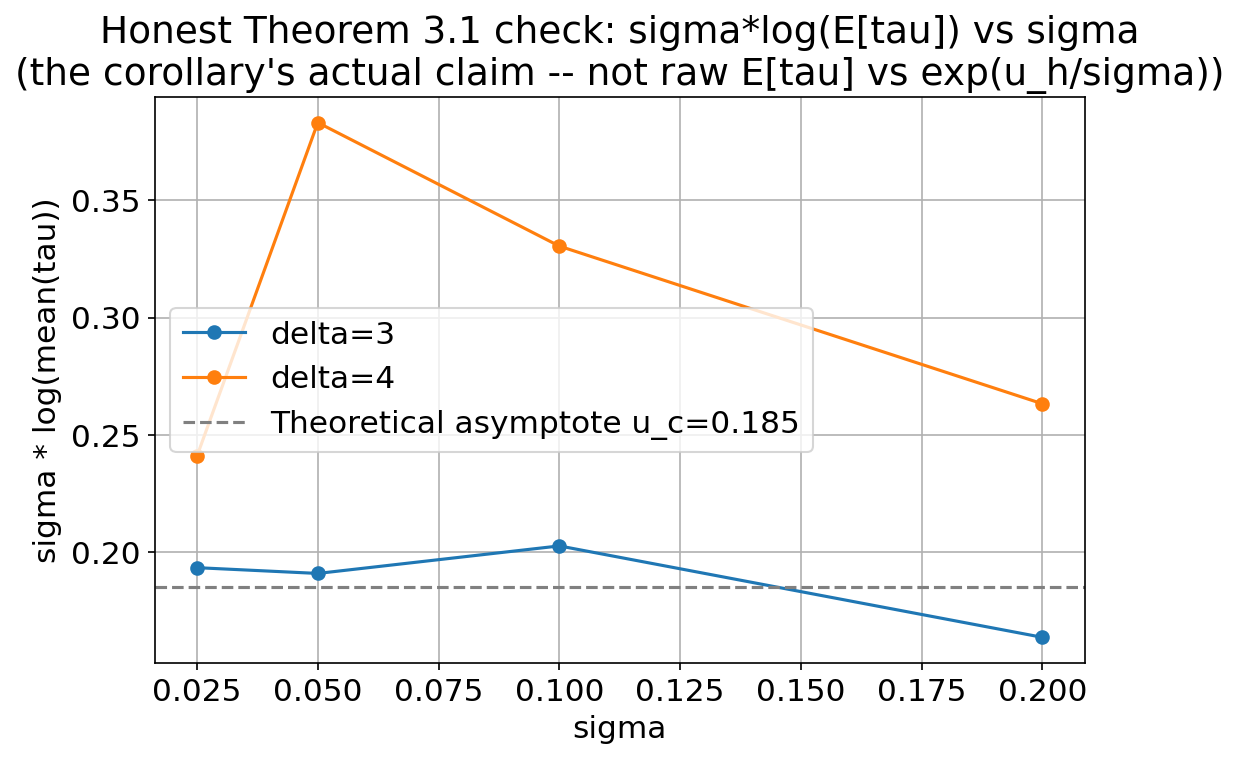
\includegraphics[width=\linewidth]{images/theory_verification_honest.png}
    \caption{$\sigma\log(\text{mean }\tau)$ vs. $\sigma$ at $\delta=3,4$, i.e.\ barrier heights $h=2.19$ and $h=3.93$ (both already in the saturated $h>r_c$ regime), against the theoretical asymptote $u_c=u(r_c,\beta,n)$. This is the quantity Corollary~\ref{cor:exit-time-conditional} would constrain ($\lim_{\sigma\to 0}\sigma\log\E[\tau]=V_\beta\le u_h$, and $u_h=u_c$ in this saturated regime) under the metastable-domain hypotheses that corollary assumes and that we do not verify here; the plot is therefore a consistency check, not a test of a proven identity. It is nonetheless the right quantity to plot, unlike a direct overlay of raw $\E[\tau]$ against $\exp(u_c/\sigma)$ at one fixed, non-vanishing $\sigma$, which conflates the proven log-asymptotic rate with an uncontrolled, $h$-dependent sub-exponential pre-factor. Both series trend toward $u_c$ as $\sigma$ shrinks, consistent with the corollary; neither is monotonic all the way down, which is expected finite-$\sigma$ behavior, not a violation.}
    \label{fig:theory}
\end{figure}

\begin{figure}[H]
    \centering
    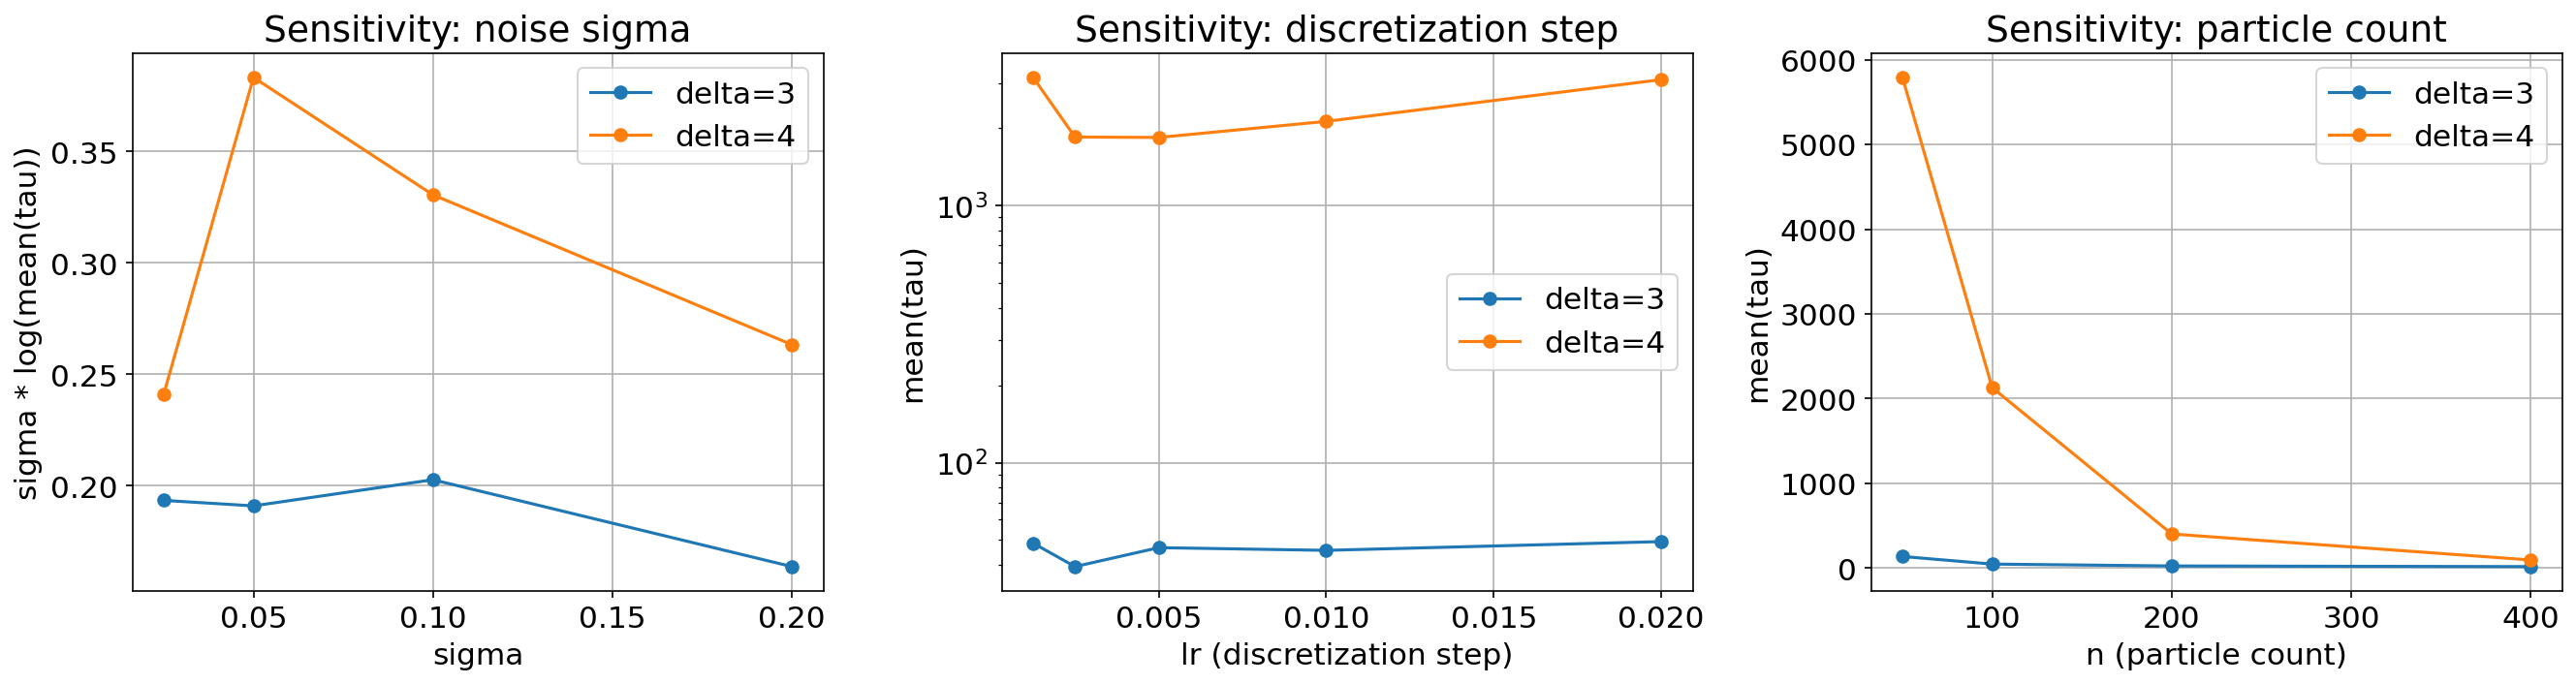
\includegraphics[width=\linewidth]{images/theory_sensitivity.png}
    \caption{Sensitivity of the same corollary check to the discretization step $\eta$ and particle count $n$, at $\delta=3,4$ ($h=2.19,3.93$). $\sigma\log(\text{mean }\tau)$ (left) reproduces Figure~\ref{fig:theory}; mean $\tau$ vs. $\eta$ (center) should flatten as $\eta\to 0$ if the discretization is close to its continuous-time limit; mean $\tau$ vs. $n$ (right) should only ever improve with more particles.}
    \label{fig:theory-sensitivity}
\end{figure}

\subsection{Computational Cost Comparison}
\label{apx:cost-comparison}

\begin{table}[H]
\centering
\caption{Mean per-particle gradient/objective evaluation counts and wall-clock time, averaged over the full double-well/quadruple-well sweep actually run (not a short synthetic probe). Counts are per-particle (n\_particles $\times$ steps), not per vectorized call. Because a run that never escapes contributes its full step budget to the average, SA's and Langevin's large counts partly reflect how often they exhaust the budget without reaching the target (Figure~\ref{fig:experiments}), not a per-step cost difference: every gradient-based method performs the same $O(n)$ work per step. Standard CBO/PSO have zero gradient evaluations by construction (gradient-free); Standard CBO's nonzero objective-evaluation count above PSO's reflects its consensus-weight computation, which re-evaluates the objective every step.}
\label{tab:cost_comparison}
\begin{tabular}{@{}lrrr@{}}
\toprule
\textbf{Method} & \textbf{Gradient Evals} & \textbf{Objective Evals} & \textbf{Wall-clock (s)} \\
\midrule
Softmin & 502{,}150 & 502{,}150 & 11.68 \\
Simulated Annealing & 14{,}149{,}330 & 14{,}149{,}330 & 351.57 \\
Langevin & 42{,}907{,}470 & 42{,}907{,}470 & 1033.74 \\
CBO & 110{,}514 & 110{,}514 & 2.79 \\
CBO Annealed & 110{,}807 & 110{,}807 & 2.79 \\
PSO & 99{,}868 & 99{,}868 & 2.43 \\
Standard CBO & 0 & 1{,}363{,}282 & 18.08 \\
Standard PSO & 0 & 99{,}852 & 1.31 \\
\bottomrule
\end{tabular}
\end{table}

\subsection{Ascent-Descent Mechanism Illustration}
\label{apx:ascent-descent-illustration}

\begin{figure}[H]
    \centering
    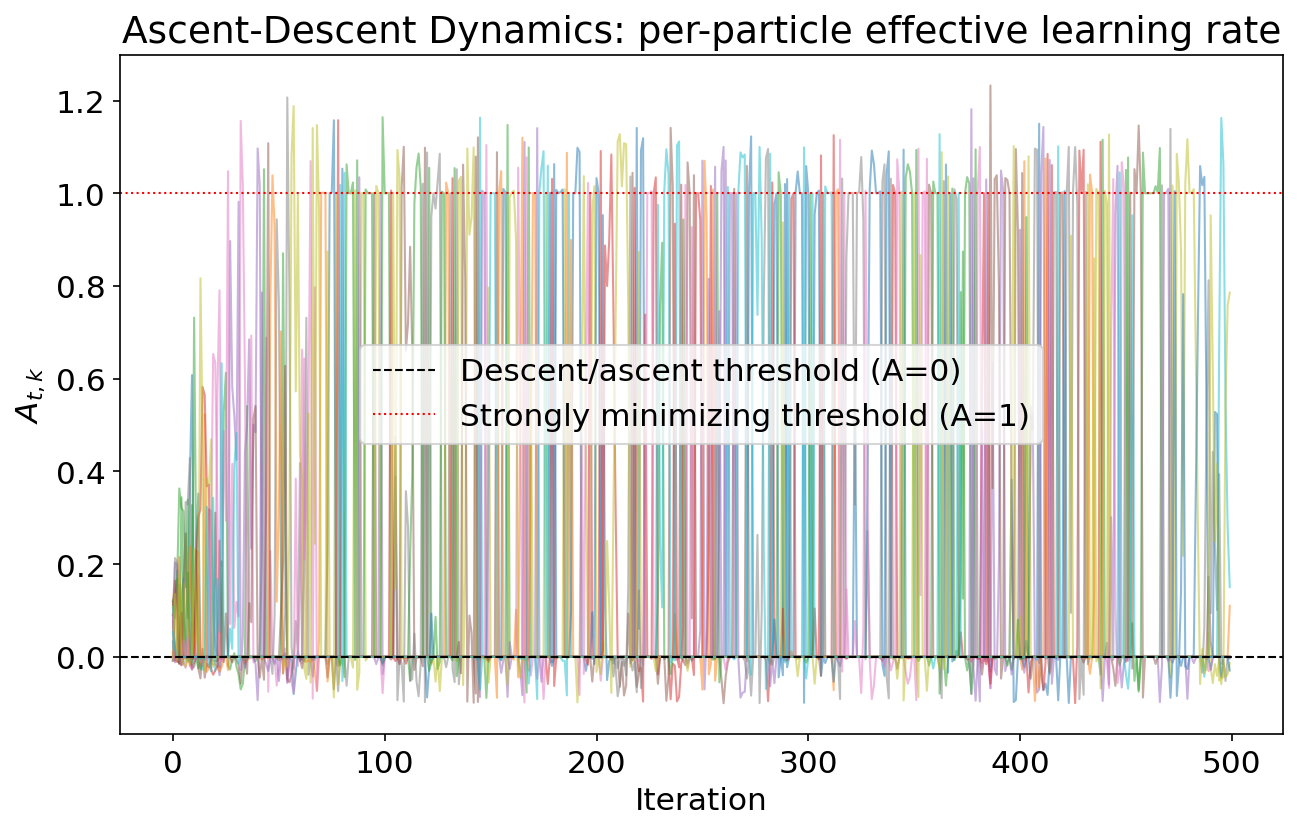
\includegraphics[width=\linewidth]{images/ascent_descent_dynamics.png}
    \caption{Per-particle effective learning rate $\prefactor{k}{\xx_t}$ over a single Softmin run on the 1D double well ($\delta=4$, i.e.\ $h=3.93$; 20 particles). Particles with $\prefactor{k}{\xx_t}>0$ descend (more strongly so above the $\prefactor{k}{\xx_t}=1$ line); particles with $\prefactor{k}{\xx_t}<0$ ascend, the mechanism the ablation study below tests directly.}
    \label{fig:ascent-descent}
\end{figure}

\subsection{Ablation Study: Ascent-Descent Mechanism}
\label{apx:ablation-study}

We isolate the contribution of the sign-changing pre-factor $\prefactor{k}{\xx}$ itself by comparing the real (\emph{signed}) mechanism against two ablations: \emph{positive part}, $(\prefactor{k}{\xx})_+$, which freezes any particle the real mechanism would have pushed uphill instead of letting it ascend; and \emph{absolute value}, $|\prefactor{k}{\xx}|$, which forces every particle to always descend, at whatever magnitude the real mechanism would have applied. All three variants share the same Gibbs/softmax weighting $n\cdot w_k$ that scales $\prefactor{k}{\xx}$ in the first place; only the sign treatment on top of it differs.

\begin{figure}[!htbp]
  \centering
  \begin{minipage}{0.48\textwidth}
    \centering
    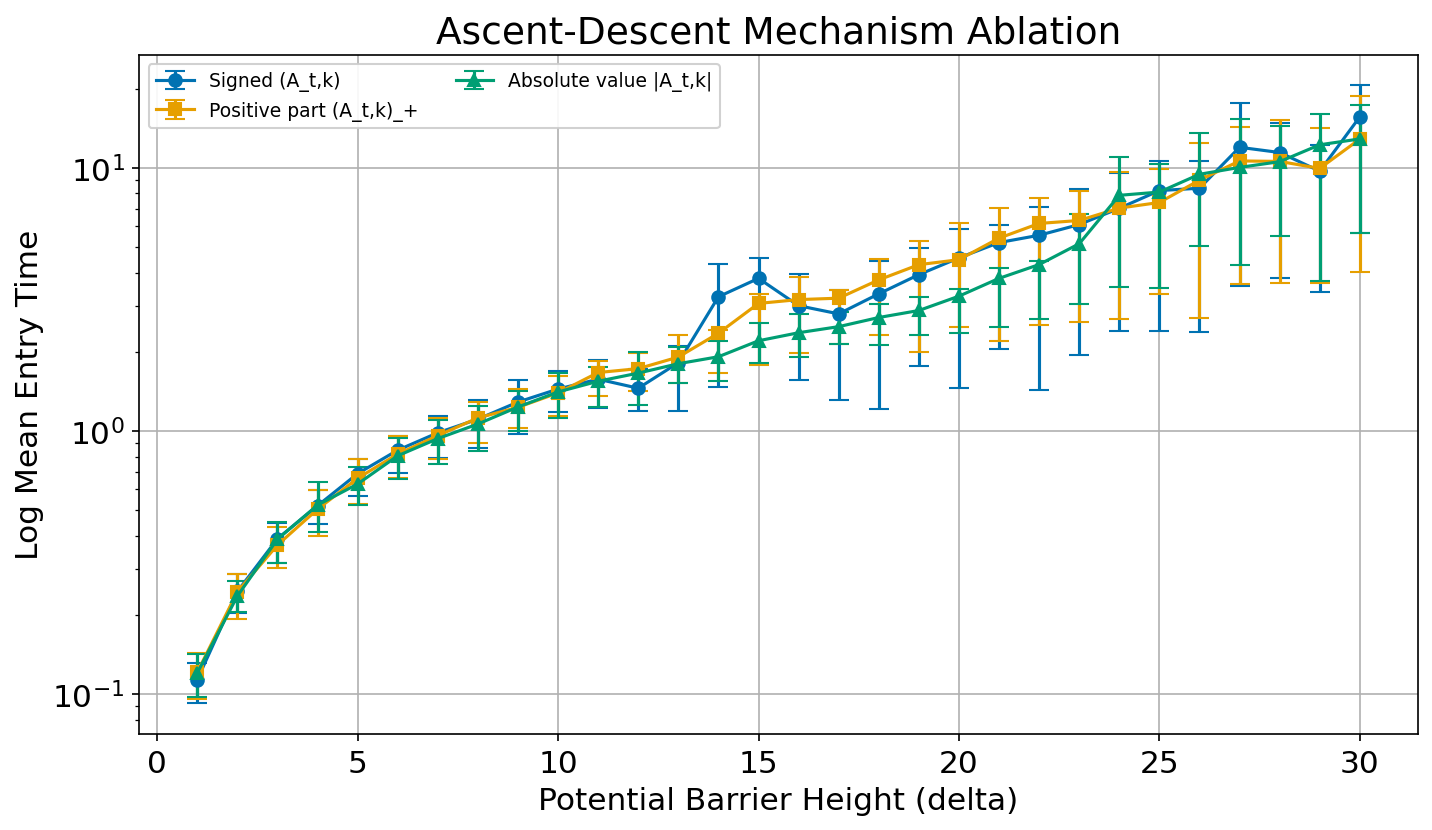
\includegraphics[width=\linewidth]{images/ablation_double_well.png}
  \end{minipage}\hfill
  \begin{minipage}{0.48\textwidth}
    \centering
    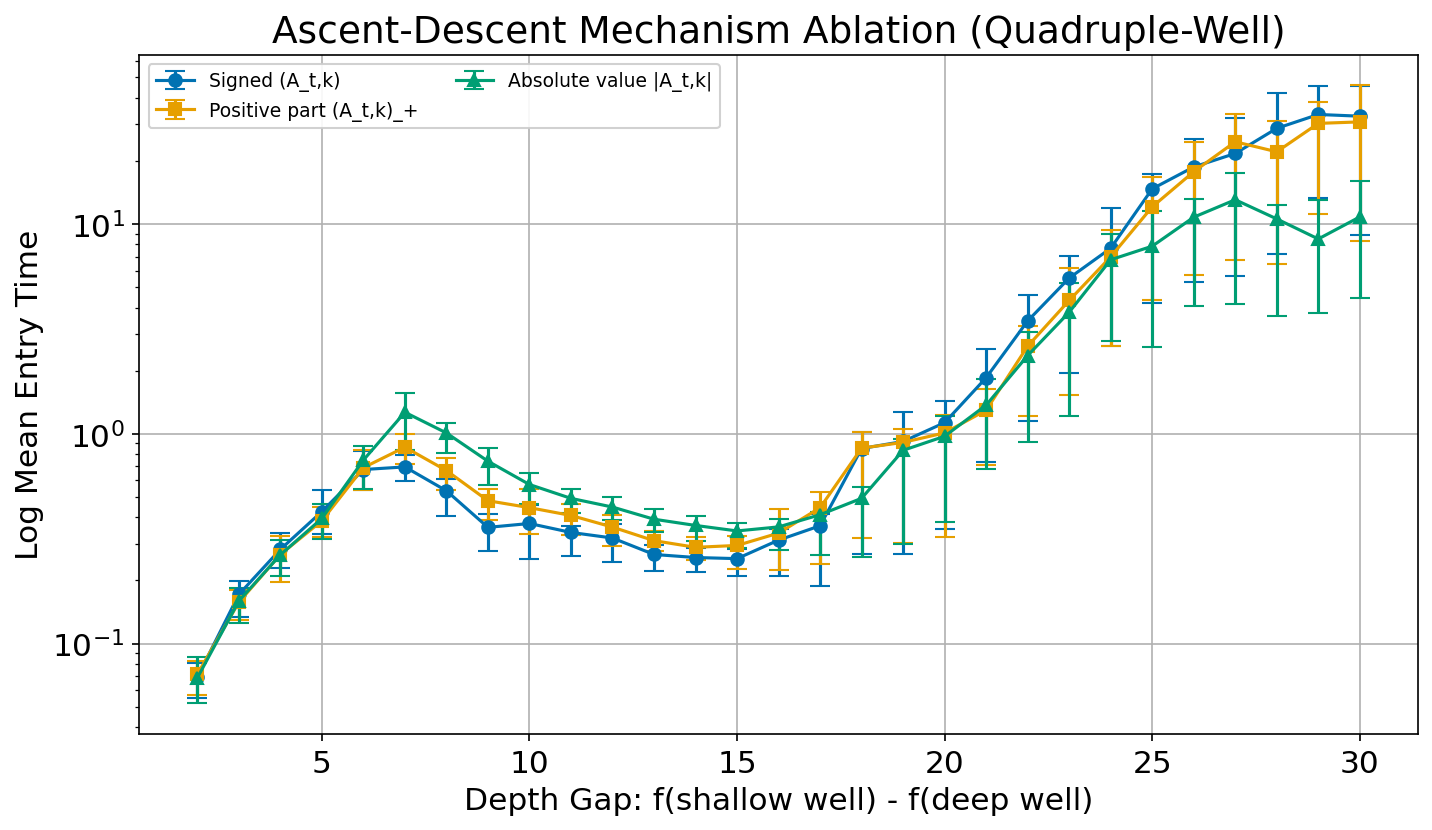
\includegraphics[width=\linewidth]{images/ablation_quadruple_well.png}
  \end{minipage}
  \caption{Ascent-descent mechanism ablation on the two swept well benchmarks (mean entry time over the seeds that reached the target, band spanning their interquartile range, vs.\ difficulty; same value-space target and status-based masking as Figure~\ref{fig:experiments}).}
  \label{fig:ablation-wells}
\end{figure}

\begin{figure}[!htbp]
  \centering
  \begin{minipage}{0.48\textwidth}
    \centering
    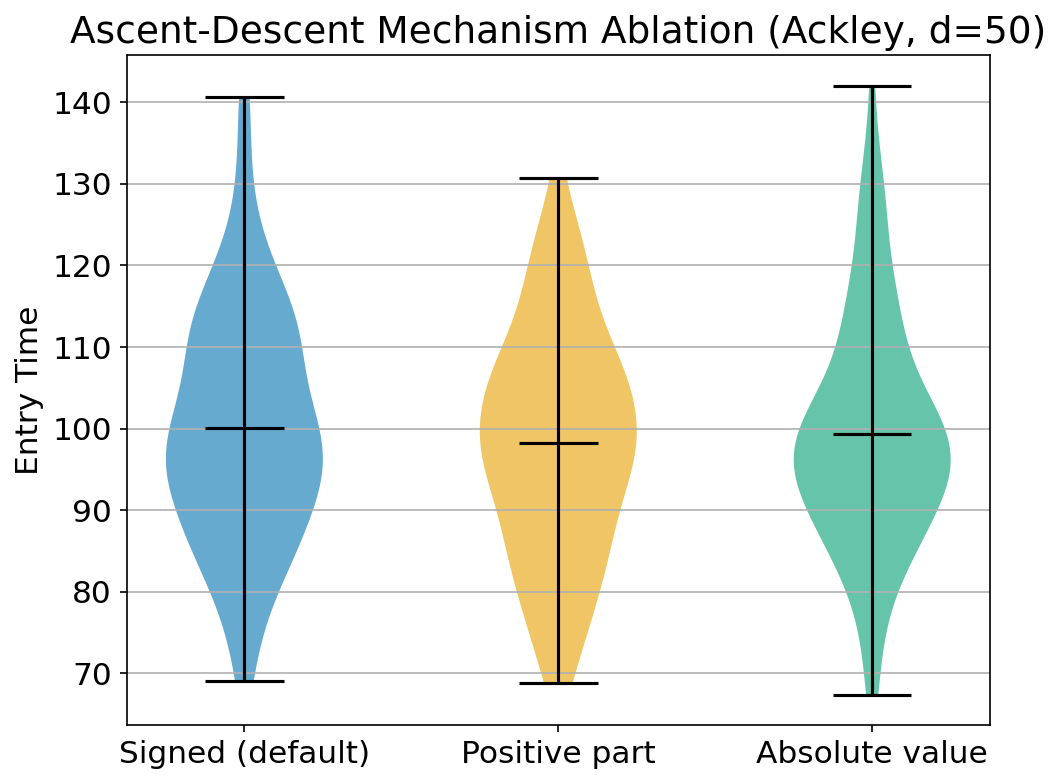
\includegraphics[width=\linewidth]{images/ablation_ackley_dim50.png}
  \end{minipage}\hfill
  \begin{minipage}{0.48\textwidth}
    \centering
    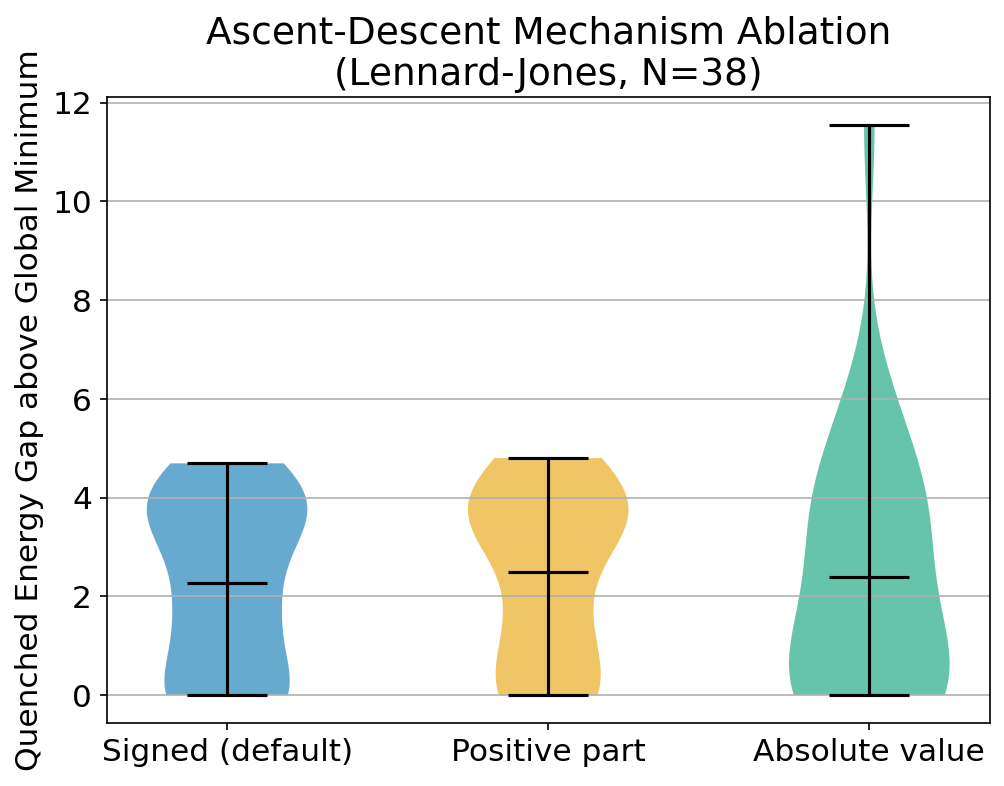
\includegraphics[width=\linewidth]{images/ablation_lj_n38.png}
  \end{minipage}
  \caption{Ascent-descent mechanism ablation at two fixed, hard settings with no natural sweep axis (Ackley $d=50$, 100 seeds; Lennard-Jones $N=38$, 30 seeds), shown as per-seed distributions (violin plots) rather than a single mean-and-interquartile-range point per mode, since the three modes turn out to substantially overlap here.}
  \label{fig:ablation-fixed}
\end{figure}

The result is not the clean "signed wins, the ablations degrade" story the sign-flipping mechanism might suggest. On the two swept well benchmarks (Figure~\ref{fig:ablation-wells}), there is no consistent winner: at the easier settings signed is competitive or best (e.g. quadruple well $A=15$: signed $0.25$, positive part $0.29$, absolute $0.34$), but at harder settings absolute is clearly faster, e.g.\ double well $\delta=15$ ($h=56.1$): signed $3.81$, positive part $3.06$, absolute $2.20$; quadruple well $A=30$: signed $32.69$, positive part $30.70$, absolute $10.82$, roughly $3\times$ faster than either alternative that still preserves or freezes the sign. At the two fixed, hard settings (Figure~\ref{fig:ablation-fixed}) the three modes are close to indistinguishable: Ackley $d=50$ entry time (mean $100.1$/$98.2$/$99.4$ for signed/positive part/absolute, all 100\% reached) and Lennard-Jones $N=38$ quenched-energy gap ($2.26$/$2.48$/$2.40$) show heavily overlapping distributions.

Taken together, these four benchmarks suggest that preserving the sign of $\prefactor{k}{\xx}$, letting trailing particles genuinely ascend rather than merely stall or be redirected downhill, is not what is doing most of the practical work in this noise regime ($\sigma=1$). The Gibbs/softmax weighting $n\cdot w_k$, identical across all three variants, already strongly suppresses trailing particles' contribution regardless of the sign convention applied on top of it; that shared attenuation is the more plausible source of the empirical advantage over the baselines on the well and Lennard-Jones benchmarks of Section~\ref{sec:numerical-experiments}. The sign-flipping ascent mechanism remains what Theorem~\ref{thm:transition-time} is stated and proved for, and is a $\sigma\to 0$ asymptotic statement; these benchmarks run at a fixed, non-vanishing $\sigma$, and the ablation results here are consistent with the sign convention mattering more as $\sigma$ shrinks than it does at the noise level tested.

\begin{figure}[H]
    \centering
    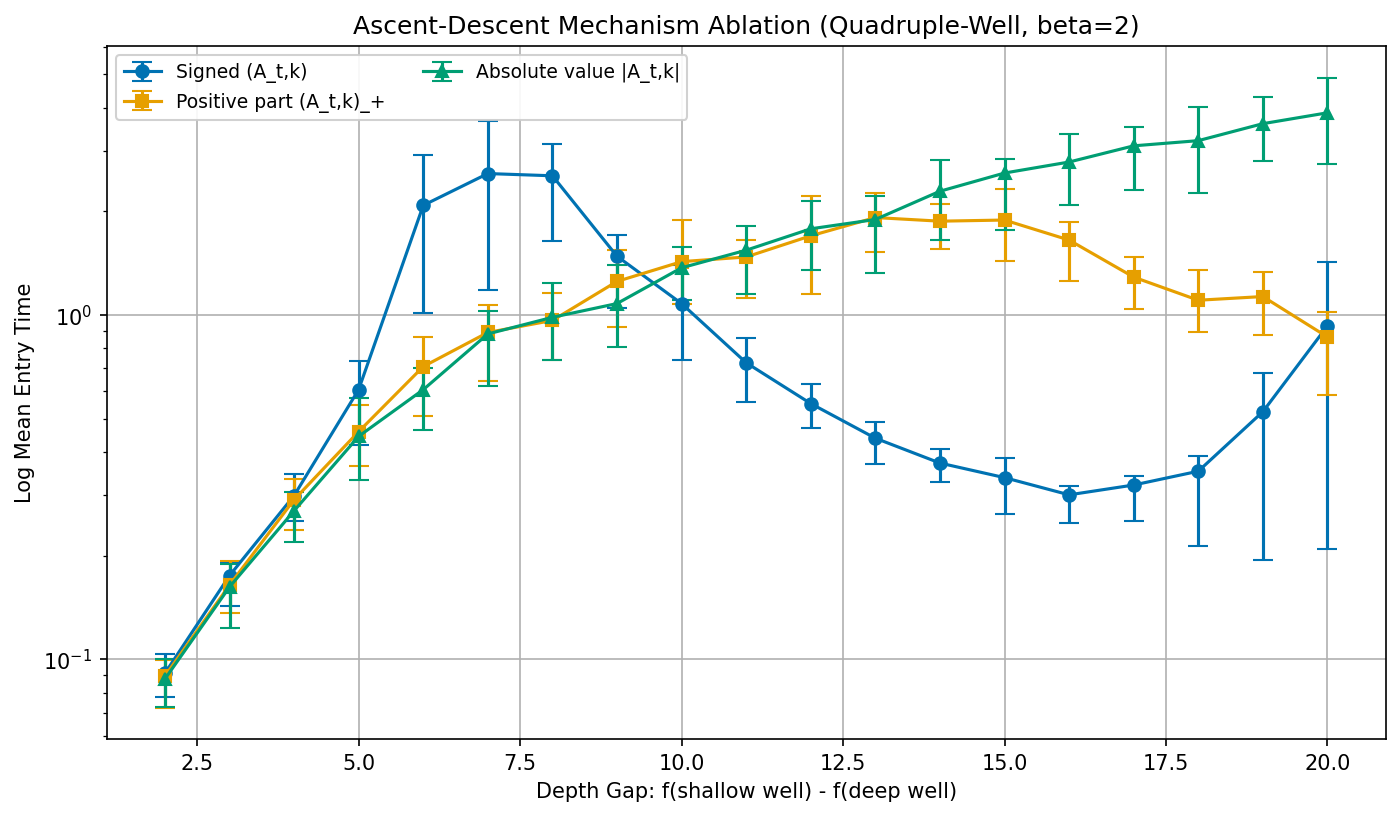
\includegraphics[width=\linewidth]{images/ablation_quadruple_well_beta2.png}
    \caption{Ascent-descent mechanism ablation on the 2D quadruple well at a lower inverse temperature ($\beta=2$, vs.\ $\beta=10$ above; 50 seeds per point, $A=2,\dots,20$), where the Gibbs weight $n\cdot w_k$ no longer concentrates sharply enough to mask the sign convention's effect.}
    \label{fig:ablation-quadruple-well-beta2}
\end{figure}

The near-parity at $\beta=10$ raises a natural question: is it specific to that aggressive a weighting? A sharply concentrated Gibbs weight already suppresses trailing particles' contribution regardless of the sign convention applied on top of it, by the argument above, so a less concentrated weighting should let the sign convention's own effect show through more directly. Repeating the quadruple-well ablation at $\beta=2$ (Figure~\ref{fig:ablation-quadruple-well-beta2}) confirms this: at the easier settings absolute and positive part are faster than signed, sometimes markedly so (depth gap $7$: signed $2.58$, positive part $0.89$, absolute $0.88$), but this reverses once the barrier grows past a depth gap of about $10$: from depth gap $13$ through $19$ signed is consistently and substantially faster (e.g.\ depth gap $15$: signed $0.34$, positive part $1.89$, absolute $2.59$; depth gap $19$: signed $0.52$, positive part $1.13$, absolute $3.60$, nearly $7\times$ faster than absolute). At this lower temperature, preserving the sign of $\prefactor{k}{\xx}$, letting trailing particles genuinely ascend rather than merely stall or be redirected downhill, becomes the decisive factor precisely as the barrier increases: as the escape genuinely gets harder, only the mechanism that lets trailing particles actively climb out keeps up, consistent with the sign-flipping mechanism Theorem~\ref{thm:transition-time} is stated and proved for.

\section{Extended Limitations and Future Work}
\label{apx:limitations}

Our theoretical analysis provides rigorous guarantees in the practically relevant small-noise regime where the Freidlin--Wentzell Large Deviation Principles apply. While the bound in Theorem~\ref{thm:transition-time} is not sharp (in particular $u_c$ and $u_h$ are only upper-estimated by an explicit channel, not computed exactly for general $f$), a tighter characterization of the true quasipotential, together with intermediate-noise asymptotics, would sharpen the picture. Our equilibrium characterization (Theorem~\ref{thm:stationary-points}) requires no convexity assumption on $f$ whatsoever; the ensemble-descent estimate (Theorem~\ref{thm:ensemble-min}) guarantees the running minimum is nonincreasing regardless, but its exponential rate of convergence specifically to the global minimum requires a Polyak--\L{}ojasiewicz condition on the relevant sublevel set. The exit-time consequence of Theorem~\ref{thm:transition-time} holds unconditionally only at the level of the quasipotential, and becomes an actual statement about $\E\tau^\sigma$ only under the unverified metastable-domain hypotheses of Corollary~\ref{cor:exit-time-conditional}; identifying the exact transition exponent between adjacent basins, and a rigorous large-deviation treatment of the annealed schedule $\beta_t$, remain open.

A second gap is empirical, between what the theory describes and what the benchmarks measure. The benchmarks run at $\sigma=1$, where the cap of \eqref{eq:barrier-cap-appendix} evaluates to $u_c\approx0.037$ and so is negligible against the noise; the ablation of Appendix~\ref{apx:ablation-study} correspondingly finds that at $\beta=10$ the sign-reversal mechanism the theory is built on is not what produces the observed advantage, with the Gibbs weighting shared by all three ablation variants the more plausible source. The mechanism does become decisive at the lower temperature $\beta=2$, precisely as barriers grow, which is the behavior the theory predicts; but establishing that the proven mechanism drives the headline results would require either running the benchmarks down toward the small-noise regime or a control that removes the drift entirely, neither of which we do here. The Ackley results bound the claim from the other side. There the sign-reversal mechanism is active, since the landscape's barriers sit well above $r_c$, and Softmin's performance improves with dimension exactly as those barriers shrink, yet PSO is faster at every dimension, on a benchmark where gradient information demonstrably contributes nothing. Barrier flattening is therefore not sufficient for competitive speed on a landscape whose difficulty is carried by the density of minima rather than by their depth. Why PSO in particular does so well here we leave open: we did not isolate the responsible mechanism, and the comparison identifies the limitation without explaining it.

Future work should address several important directions. First, extending convergence proofs and explicit convergence rates to the non-convex regime, particularly for objectives with multiple disconnected basins, would significantly broaden applicability. Second, analyzing the mean-field limit as $n \to \infty$ could provide insights into the scaling of the method with ensemble size and potentially yield dimension-free convergence rates. Third, although Theorem~\ref{thm:ensemble-min} guarantees the ensemble-descent bound for an arbitrary schedule $\beta_t$, our experiments (Remark~\ref{rem:higher-dim}) found that neither a decaying nor an increasing schedule improved on a well-chosen fixed $\beta$ on the benchmarks considered, contrary to the original motivation for annealing $\beta$ over time; understanding whether this is a property of these specific landscapes or a more general phenomenon, and whether an adaptive schedule driven by the ensemble's own state (rather than a fixed function of $t$) can do better, is an open, concrete direction. Finally, tighter estimates for the exponential rate in the small noise regime can sharpen the theoretical bound to match experimental evidence more closely.

\end{document}
